\documentclass[a4paper, 11pt]{scrartcl}

\usepackage[utf8]{inputenc}
\usepackage[T1]{fontenc}
\usepackage{graphicx, wrapfig}
\usepackage{geometry}
\geometry{top=3cm, left = 3cm, right=3cm, bottom=3cm}
\usepackage{lmodern}
\usepackage{fancyhdr}
\usepackage{color, colortbl}
\usepackage{booktabs}
\usepackage[usenames, svgnames]{xcolor}
\usepackage{amsmath, amssymb, mathrsfs, amsthm, thmtools}
\usepackage[framemethod=tikz]{mdframed}
\usepackage{pgf, pgfplots, tikz}
\usepackage{hyperref}
\usepackage{makeidx}
\usepackage[inline]{enumitem}
\usepackage[english]{babel}


\newcommand{\N}{\mathbb{N}}
\newcommand{\Q}{\mathbb{Q}} 
\newcommand{\R}{\mathbb{R}}
\newcommand{\Z}{\mathbb{Z}} 
\newcommand{\C}{\mathbb{C}}
\newcommand{\K}{\mathbb{K}}
\renewcommand{\epsilon}{\varepsilon}
\renewcommand{\phi}{\varphi}
\renewcommand{\emph}{\textbf}



%%%%%%%%	Définitions des environnements des exercices	%%%%%%%%
%----- ENVIRONNEMENT POUR LES EXERCICES ----%
\declaretheoremstyle[
  spaceabove=0pt, spacebelow=0pt, headfont=\normalfont\bfseries\scshape,
    notefont=\mdseries, notebraces={(}{)}, headpunct={. }, headindent={},
    postheadspace={ }, postheadspace=4pt, bodyfont=\normalfont, %qed=$$,
    mdframed={
      leftmargin=-5,
      rightmargin=-5,
      hidealllines=true
   }
]{defstyle}

\declaretheorem[style=defstyle, title=Exercice]{ex}
%________________________________________________________


%----- ENVIRONNEMENT POUR LES SOLUTIONS ----%
\declaretheoremstyle[
  spaceabove=-10pt, spacebelow=0pt, headfont=\normalfont\scshape,
    notefont=\mdseries, notebraces={(}{)}, headpunct={. }, headindent={},
    postheadspace={ }, postheadspace=4pt, %bodyfont=\normalfont, 
    qed=\qedsymbol,
    mdframed={
      leftmargin=15,
      rightmargin=15,
      hidealllines=true,
      font=\small
   }
]{preuvestyle}

\declaretheorem[style=preuvestyle, numbered=no, title=Solution]{sol}

\synctex=1

\addtokomafont{disposition}{\normalfont\bfseries}

\title{\vspace{-1cm}\normalfont{\bfseries{Probabilistic Algorithms Project \\ {\Large Comparing heuristics for
      TSP}}}}
\author{Laurent \textsc{Hayez}}
\date{\today}% Date de création: 27 mars 2015\\ Dernière modification: \today}

\pagestyle{fancy}
\fancyhead[L]{Université de Neuchâtel}
\fancyhead[R]{Laurent Hayez}



\begin{document}


\renewcommand{\labelitemi}{\textbullet}

\maketitle

\thispagestyle{fancy}



\section{Introduction}

The Traveling Salesman Problem (TSP) is an old problem, having written sources as old as almost 300 years. The
problem consists of a person needing to visit $n$ cities, but with constraints. The constraints are that the
person must visit each of the $n$ cities only once, and must do it in an optimal way, i.e., the total
traveled distance must be the smallest possible.

This problem is hard to solve deterministically. Indeed, to find the optimal solution, we would need to test
every possible path in the graph composed of the $n$ cities, and the paths between them. If there are $n$
cities, the number of paths to test is $n!$, and the computations become impractical when $n$ is as small as
$20$. 

This hardness justifies the need to use heuristics, and probabilistic algorithms to solve the problem. Of
course, there is no guarantee that we will find the optimal path, but the heuristics return good enough
paths. The goal of this project is to compare a few heuristics that can be used to solve the TSP. We will
compare the best solutions found by each algorithms, the differences for the routes, the performance of the
algorithms, and pairwise statistical comparison of the algorithms. 

\section{Comparison of loss values}

Denote by $\mathcal{L}$ the sequence $\{L(\sigma_1^{\ast}), \ldots, L(\sigma_m^{\ast})\}$ of the best
solutions generated after calling each implemented algorithms $m = 30$ times. We will present tables showing
the minimum of $\mathcal{L}$, the maximum, the average and the $95\%$ condidence interval for this average for
each implemented algorithms.

\begin{table}[h]
\centering
\caption{Construction heuristics}
\label{table:construction-heuristics}
\begin{tabular}{@{}lllll@{}}
\toprule
Algorithms     & $\min(\mathcal{L})$ & $\max(\mathcal{L})$ & $\mathrm{mean}(\mathcal{L})$ & Confidence interval at 95\% \\ \midrule
best insertion & 1470.1821           & 1563.2285           & 1516.5628                    & {[}1506.6866, 1526.4391{]}  \\
shortest edge  & 1584.0766           & 1753.079            & 1671.8119                    & {[}1656.668, 1686.9558{]}   \\ \bottomrule
\end{tabular}
\end{table}


\begin{table}[h]
\centering
\caption{Greedy local search}
\label{table:greedy-local-search}
\begin{tabular}{@{}lllll@{}}
\toprule
Algorithms  & $\min(\mathcal{L})$ & $\max(\mathcal{L})$ & $\mathrm{mean}(\mathcal{L})$ & Confidence interval at 95\% \\ \midrule
swap        & 1459.2188           & 1557.0646           & 1506.8777                    & [1497.346, 1516.4094]  \\
translation & 1443.1734           & 1513.6743           & 1483.3338                    & [1476.954, 1489.7137]   \\
inversion   & 1441.9932           & 1538.6809           & 1486.538                     & [1477.6003, 1495.4757]  \\
mixed       & 1417.9906           & 1497.824            & 1457.8618                    & [1451.398, 1464.3255]   \\ \bottomrule
\end{tabular}
\end{table}


\begin{table}[h]
\centering
\caption{Simulated annealing with Metropolis criterion}
\label{table:simulated-annealing-metropolis}
\begin{tabular}{@{}lllll@{}}
\toprule
Algorithms  & $\min(\mathcal{L})$ & $\max(\mathcal{L})$ & $\mathrm{mean}(\mathcal{L})$ & Confidence interval at 95\% \\ \midrule
swap        & 1480.4799           & 1570.6594           & 1524.4871                    & [1515.8524, 1533.1217]  \\
translation & 1496.309            & 1593.6313           & 1526.9437                    & [1517.9352, 1535.9522]   \\
inversion   & 1482.4386           & 1548.8955           & 1517.5976                    & [1510.4491, 1524.746]  \\
mixed       & 1484.3271           & 1570.1874           & 1520.7171                    & [1512.8956,1528.5386]  \\ \bottomrule
\end{tabular}
\end{table}

\begin{table}[!h]
\centering
\caption{Simulated annealing with heat bath condition}
\label{table:simulated-annealing-heatbath}
\begin{tabular}{@{}lllll@{}}
\toprule
Algorithms  & $\min(\mathcal{L})$ & $\max(\mathcal{L})$ & $\mathrm{mean}(\mathcal{L})$ & Confidence interval at 95\% \\ \midrule
swap        & 1475.0552           & 1592.2256           & 1530.0634                    & [1520.7394, 1539.3875]  \\
translation & 1482.6547           & 1557.8635           & 1525.6696                    & [1518.2635, 1533.0756]   \\
inversion   & 1473.0003           & 1567.3859           & 1516.8026                    & [1509.7888, 1523.8164]  \\
mixed       & 1474.1733           & 1576.7916           & 1513.6764                    & [1504.5419, 1522.8109]  \\ \bottomrule
\end{tabular}
\end{table}

We notice that the shortest edge heuristic is not good compared to the best insertion heuristic. The worst
solution found by the best insertion heuristic is still better than the best solution found by the shortest
edge heuristic. After multiple runs, the results do not come from unlucky runs, as every run resulted in
approximately the same values. It could be either because there is a mistake in the implementation of the
shortest edge heuristic, or the heuristic is not good enough. The approach is similar to the nearest neighbor
heuristic, and we know for a fact that the nearest neighbor approach does not necessarily yield good
approximations, and we can make the paths arbitrarily longer than the optimal one. 

The improvement heuristics (greedy local search and simulated annealing) all had their first solution coming
from the best insertion construction heuristic. We see for the greedy local search that the swap approach has
the worst results, but we still see an improvement compared to just using the best insertion heuristic. The
translation and inversion moves yield similar results on average. We see that the mixed approach provides the
best improvement, as it reduces the path length the most.

The Simulated Annealing algorithm with both conditions has approximately the same results, even though it
seems that the heat bath condition with mixed small moves yields the best results. The greedy local search
returns better results than the SA algorithm.



\section{Trace of best solution}
\label{sec:trace-best-solution}

\begin{figure}[!ht]
  \centering
  \begin{tabular}{cc}
    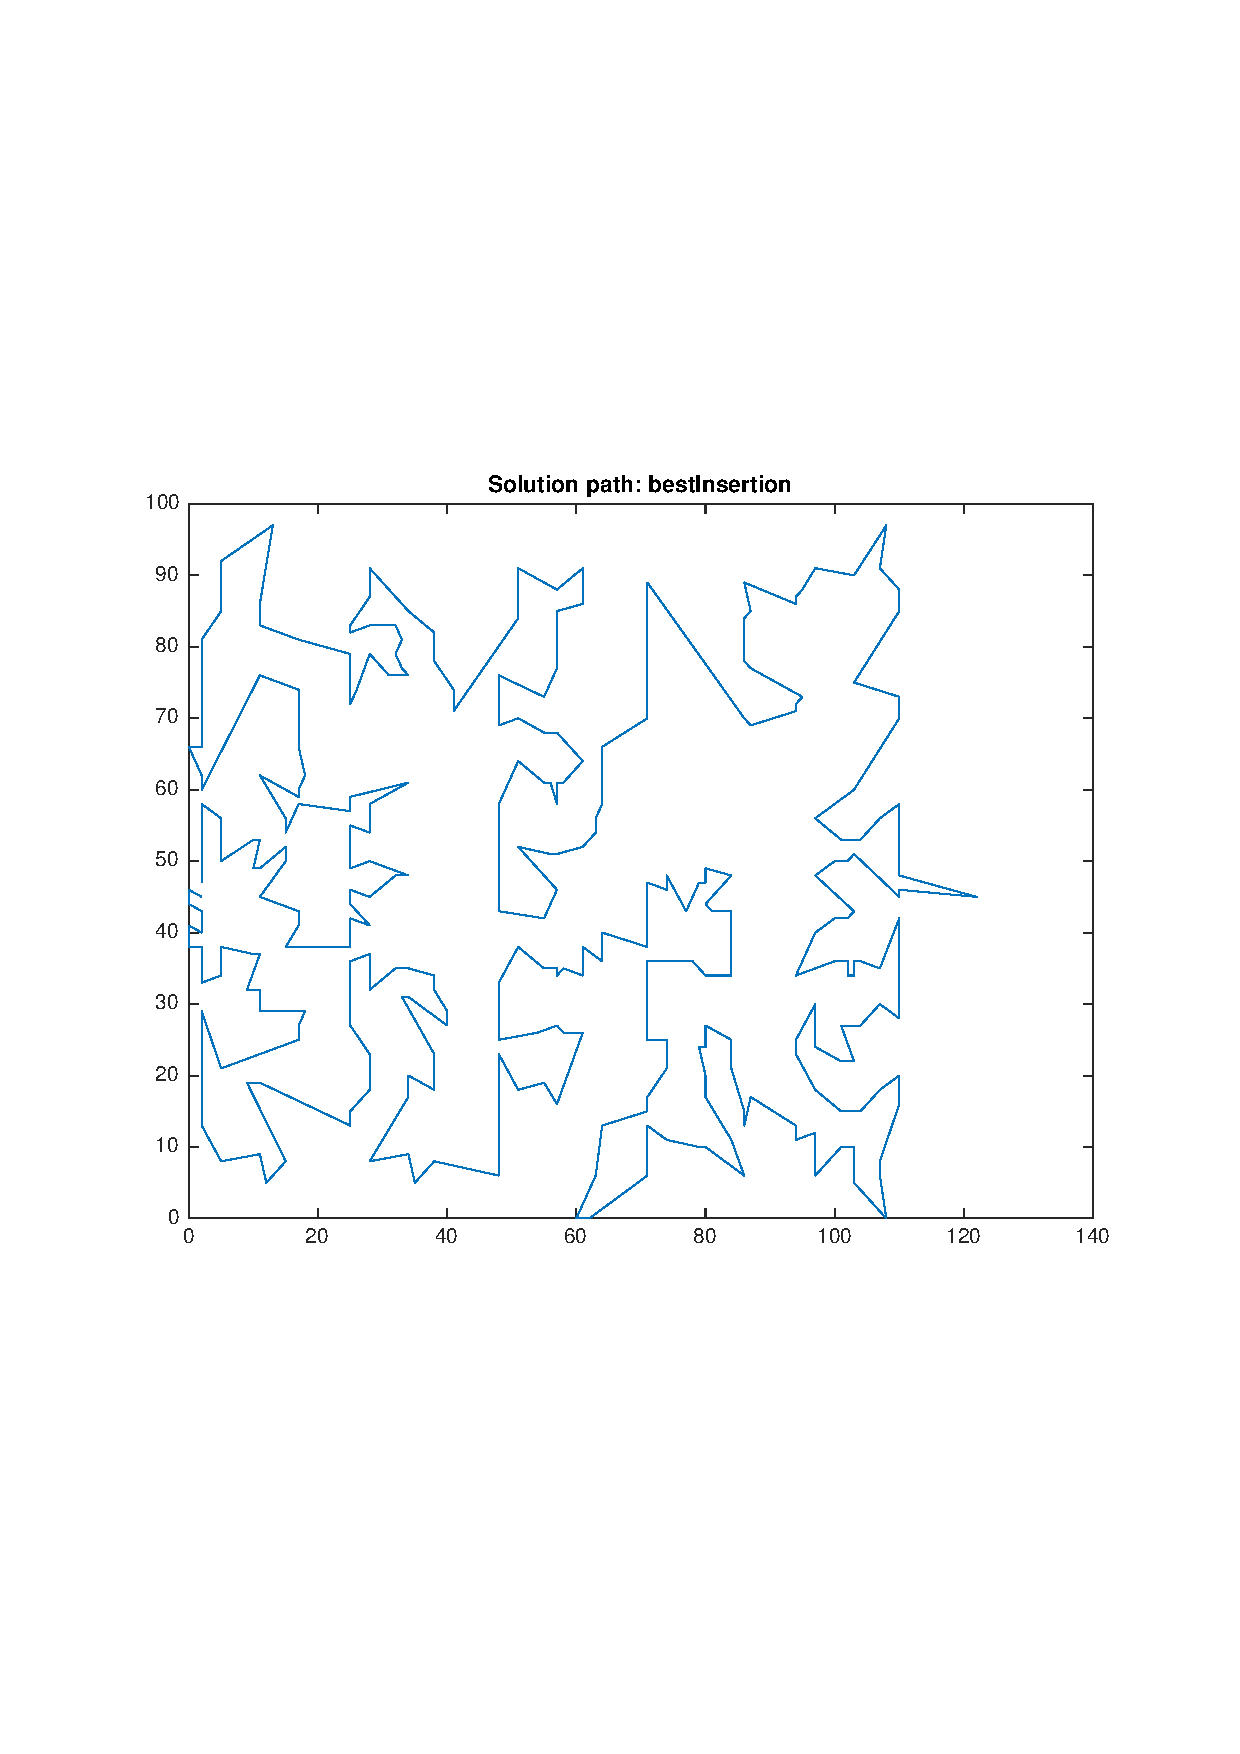
\includegraphics[scale=0.4, trim={3cm 6cm 1cm 6cm}]{../figures/solutionPath_bestInsertion.pdf} & 
    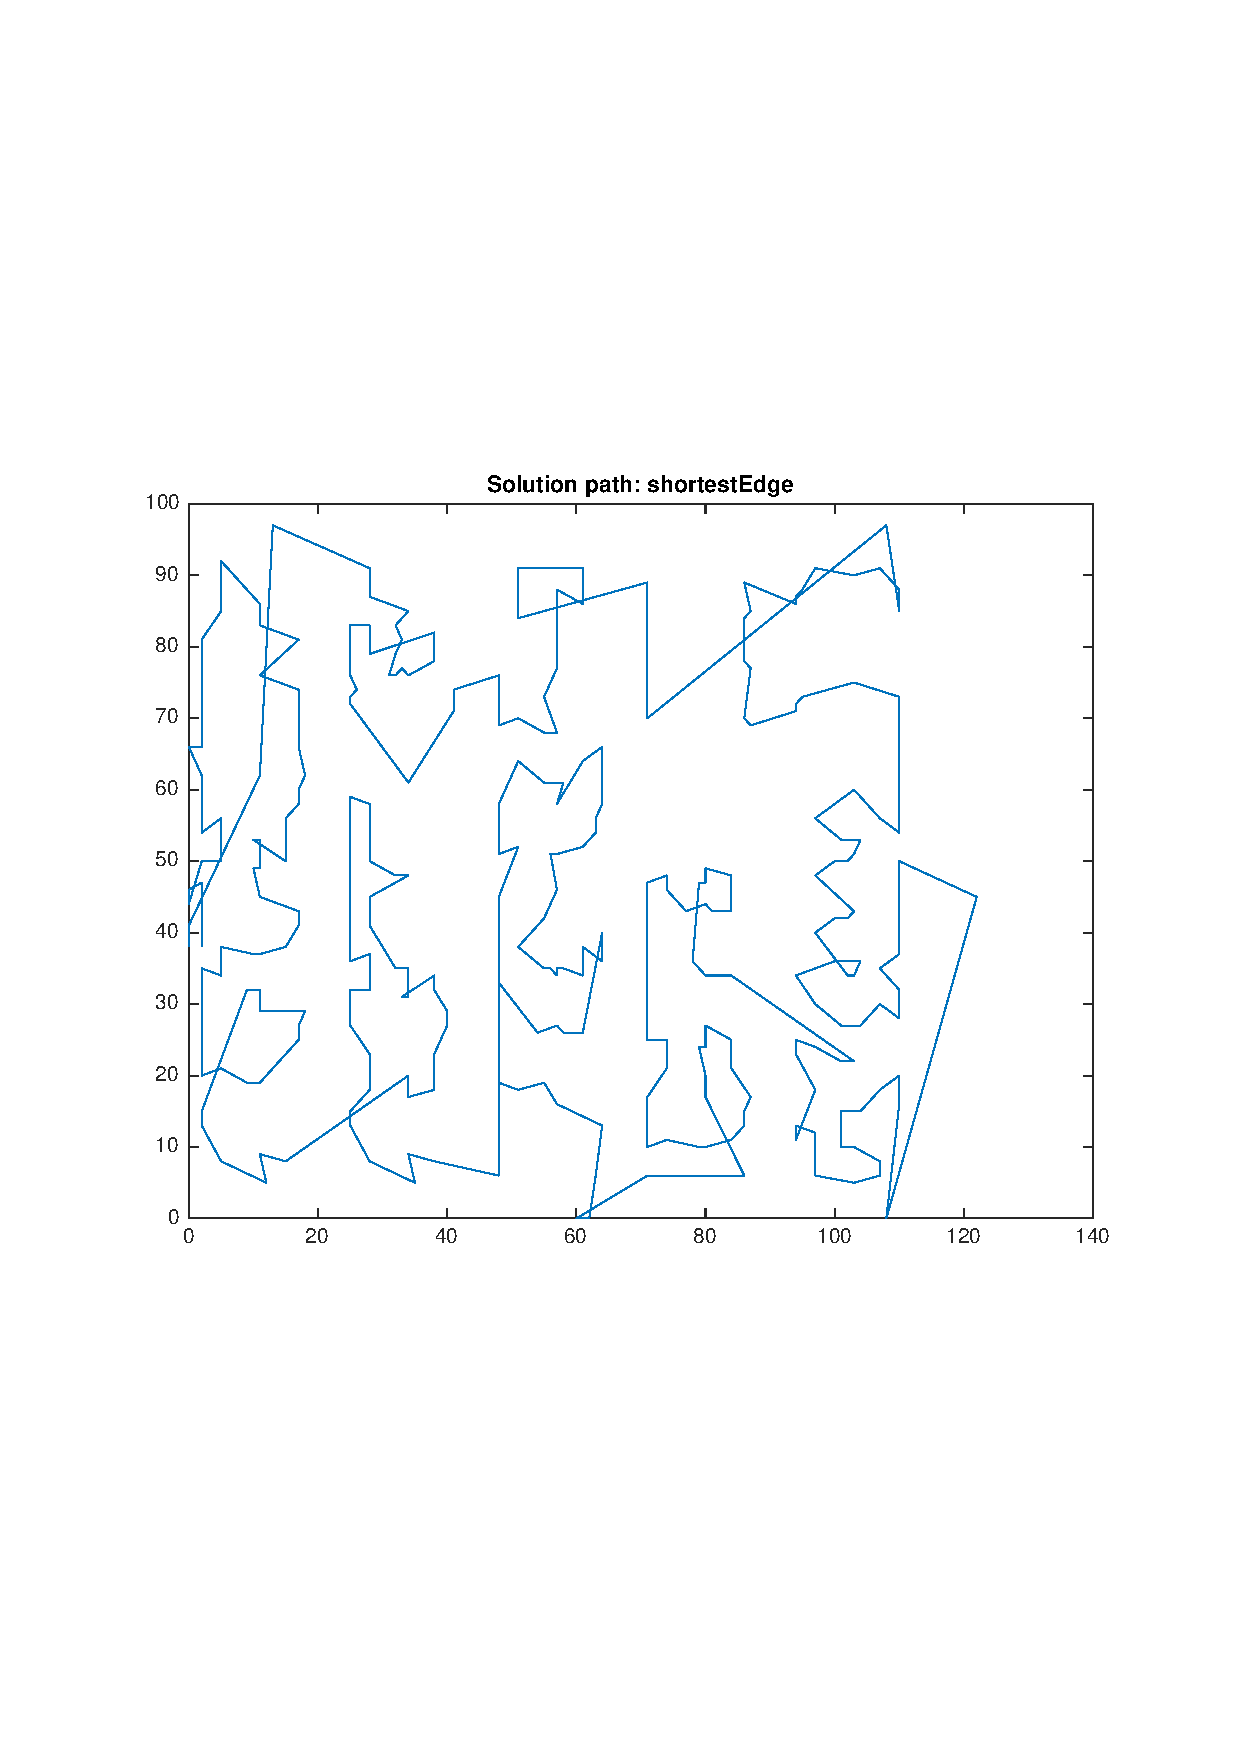
\includegraphics[scale=0.4, trim={3cm 6cm 1cm 6cm}]{../figures/solutionPath_shortestEdge.pdf}                                                                        
  \end{tabular}
  \caption{Solution path for best insertion and shortest edge heuristics}
  \label{fig:solpath-bestinsertion}
\end{figure}

\begin{figure}[!ht]
  \centering
  \begin{tabular}{cc}
    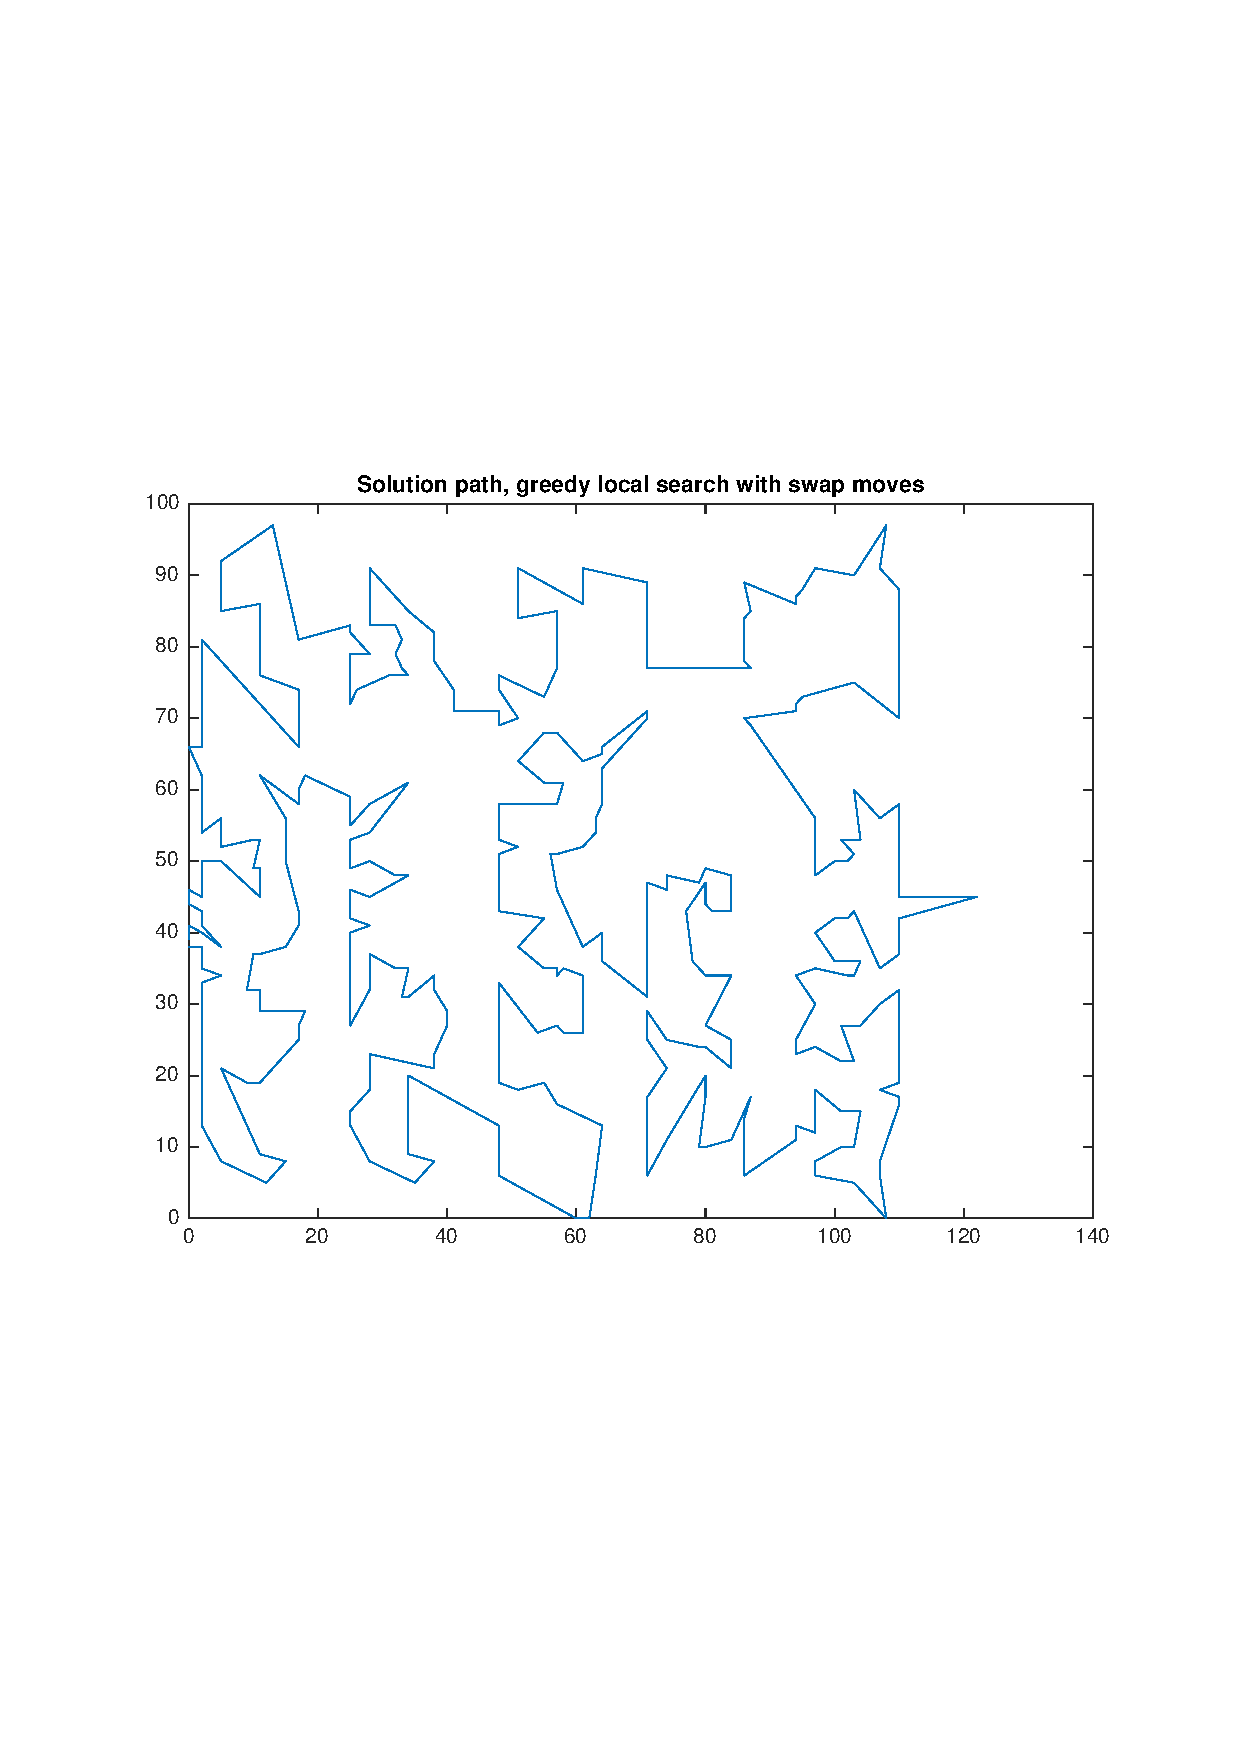
\includegraphics[scale=0.4, trim={3cm 6cm 1cm 6cm}]{../figures/solutionPath_swap.pdf} & 
    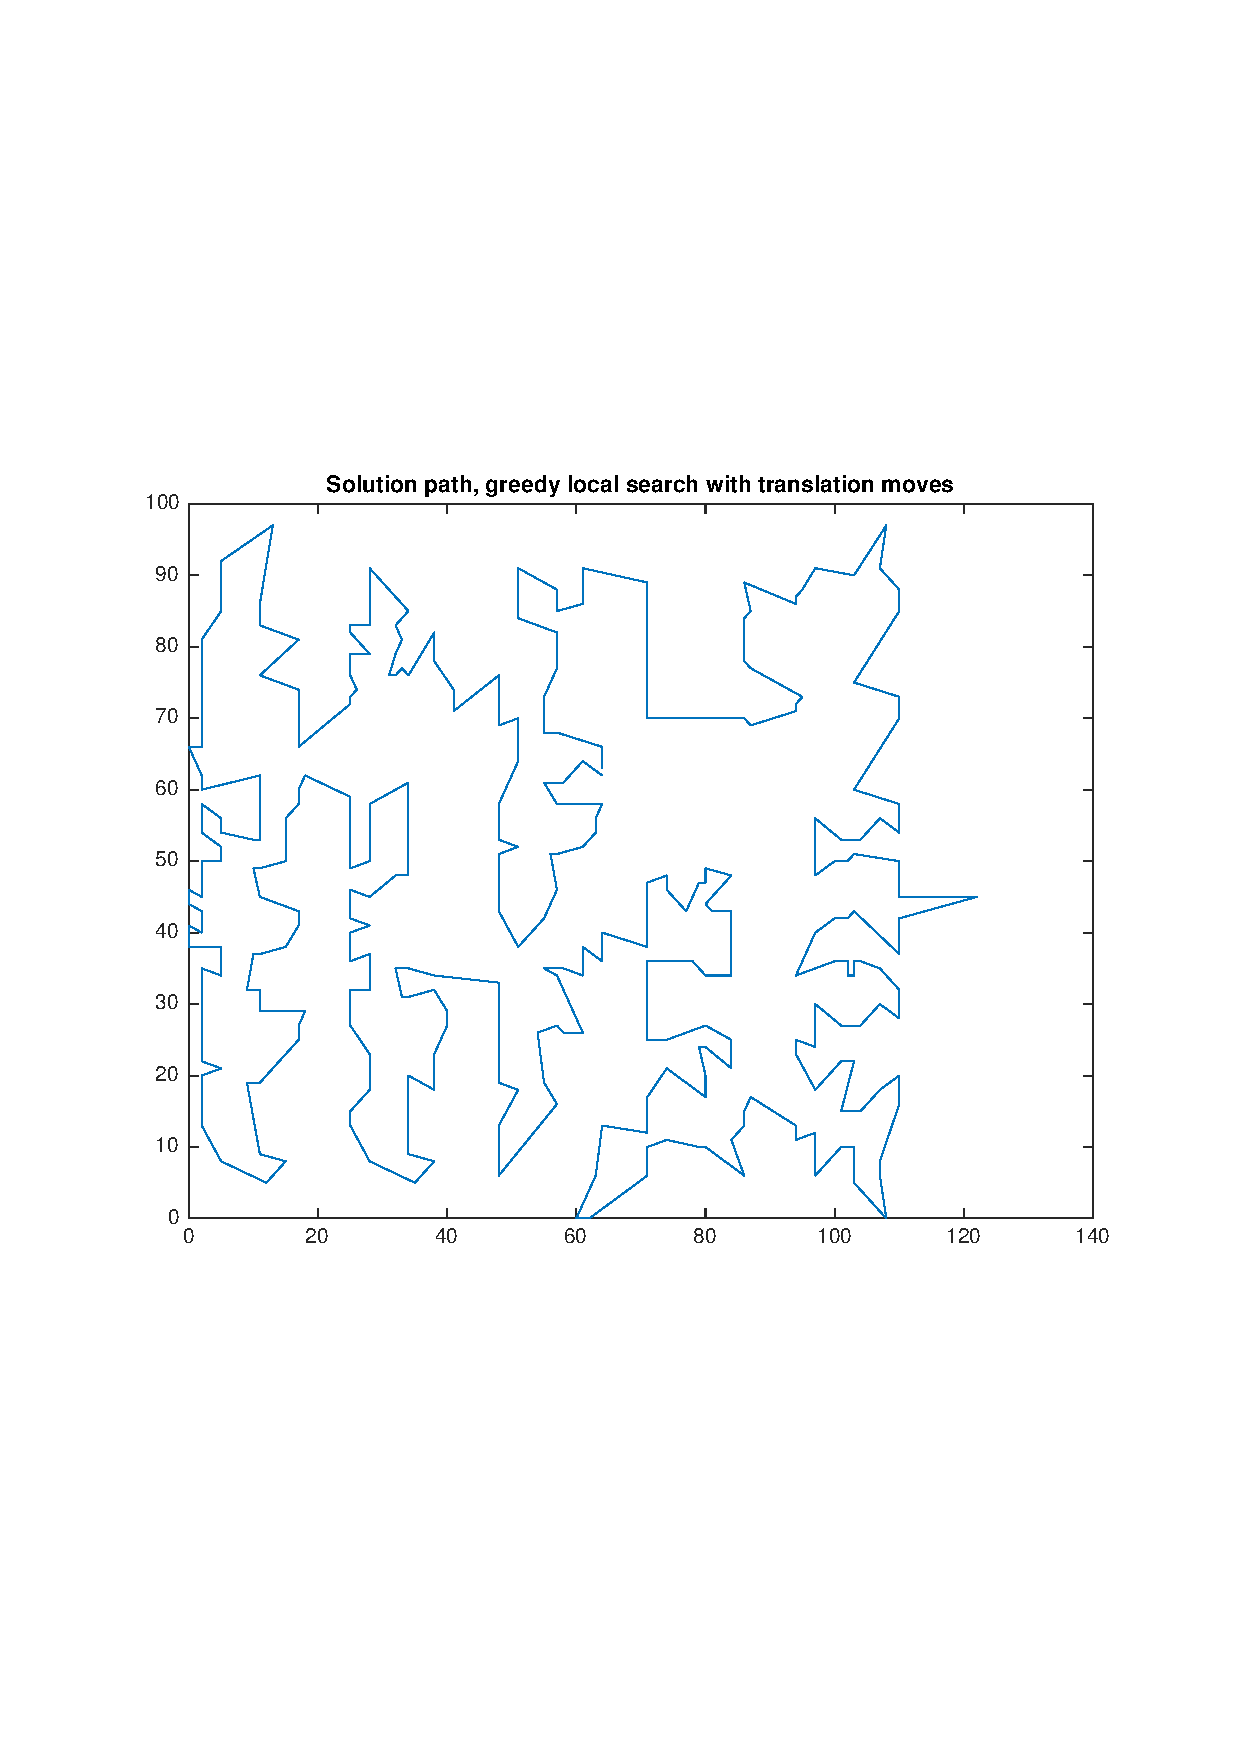
\includegraphics[scale=0.4, trim={3cm 6cm 1cm 6cm}]{../figures/solutionPath_translation.pdf} \\ 
    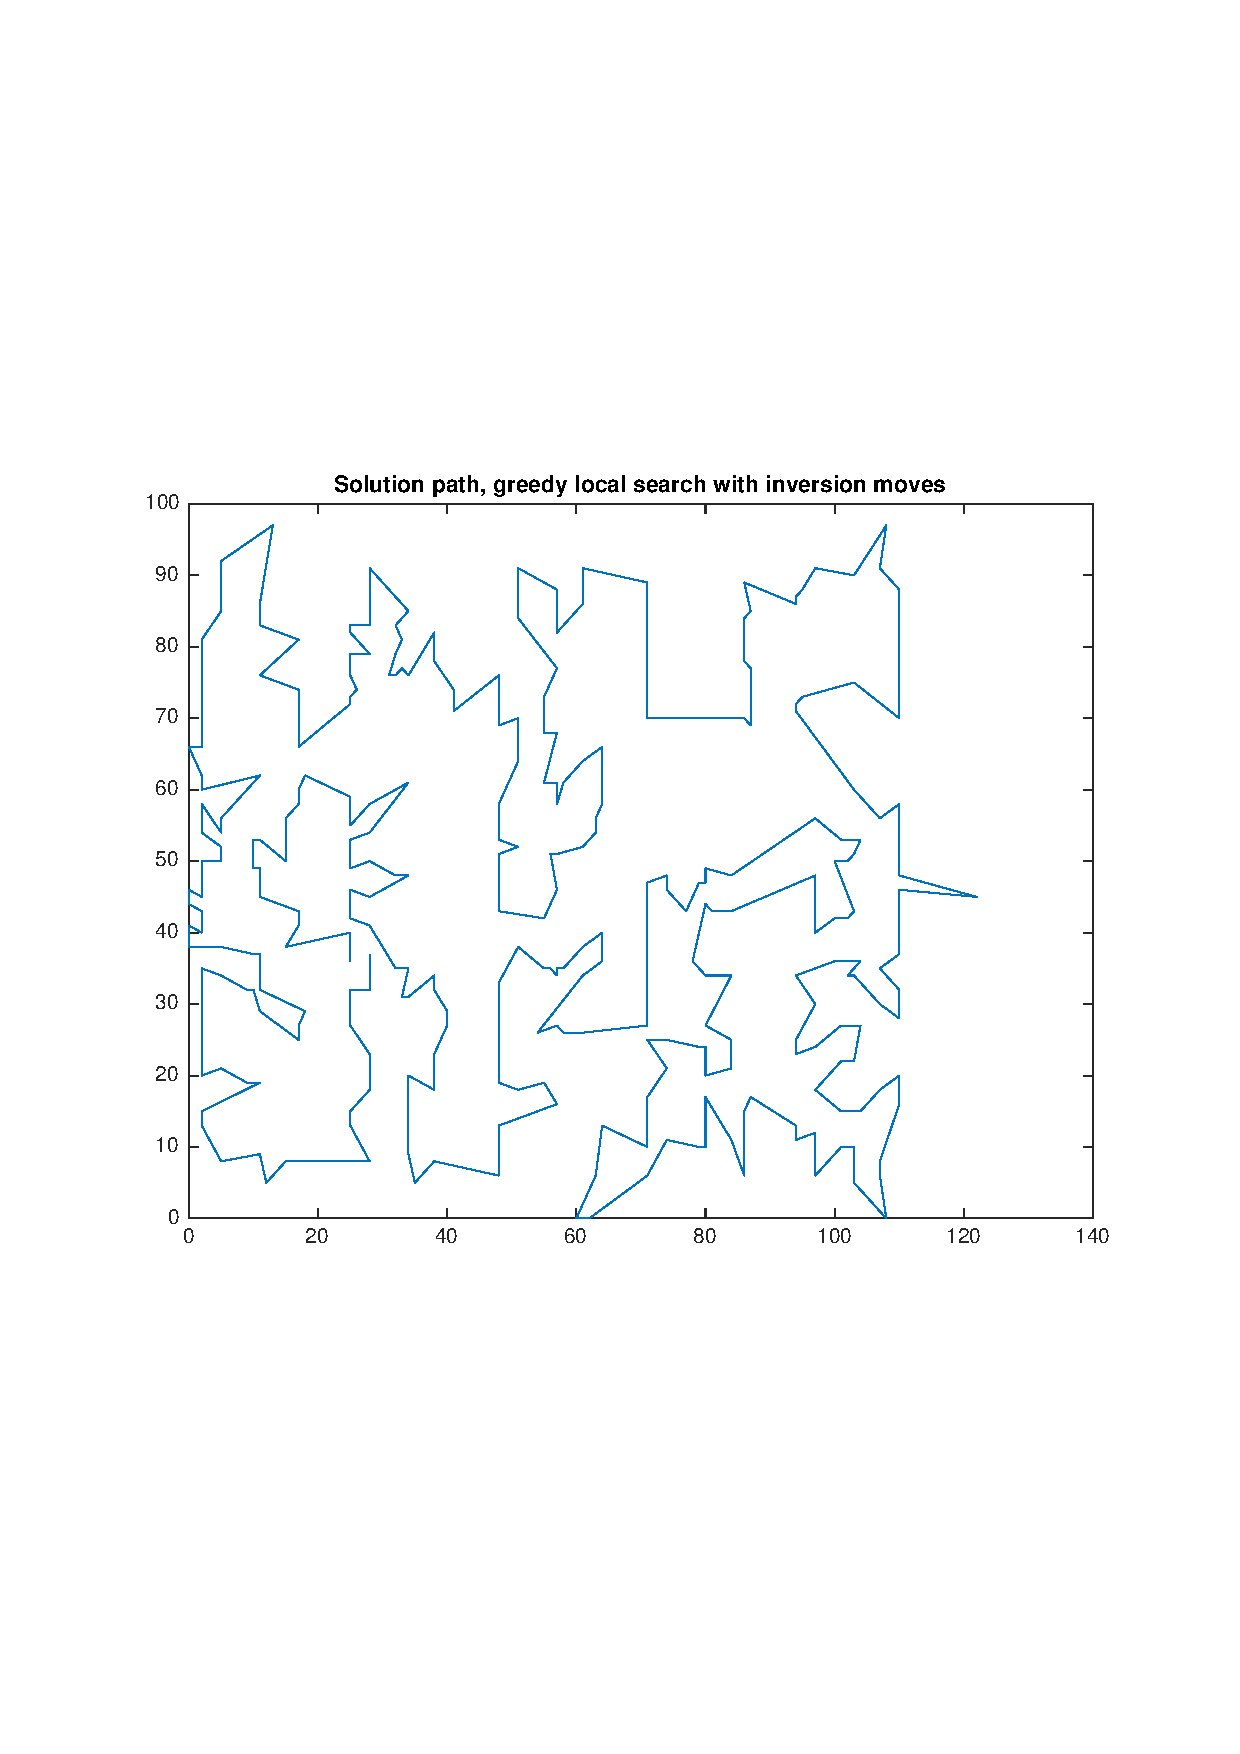
\includegraphics[scale=0.4, trim={3cm 6cm 1cm 6cm}]{../figures/solutionPath_inversion.pdf} & 
    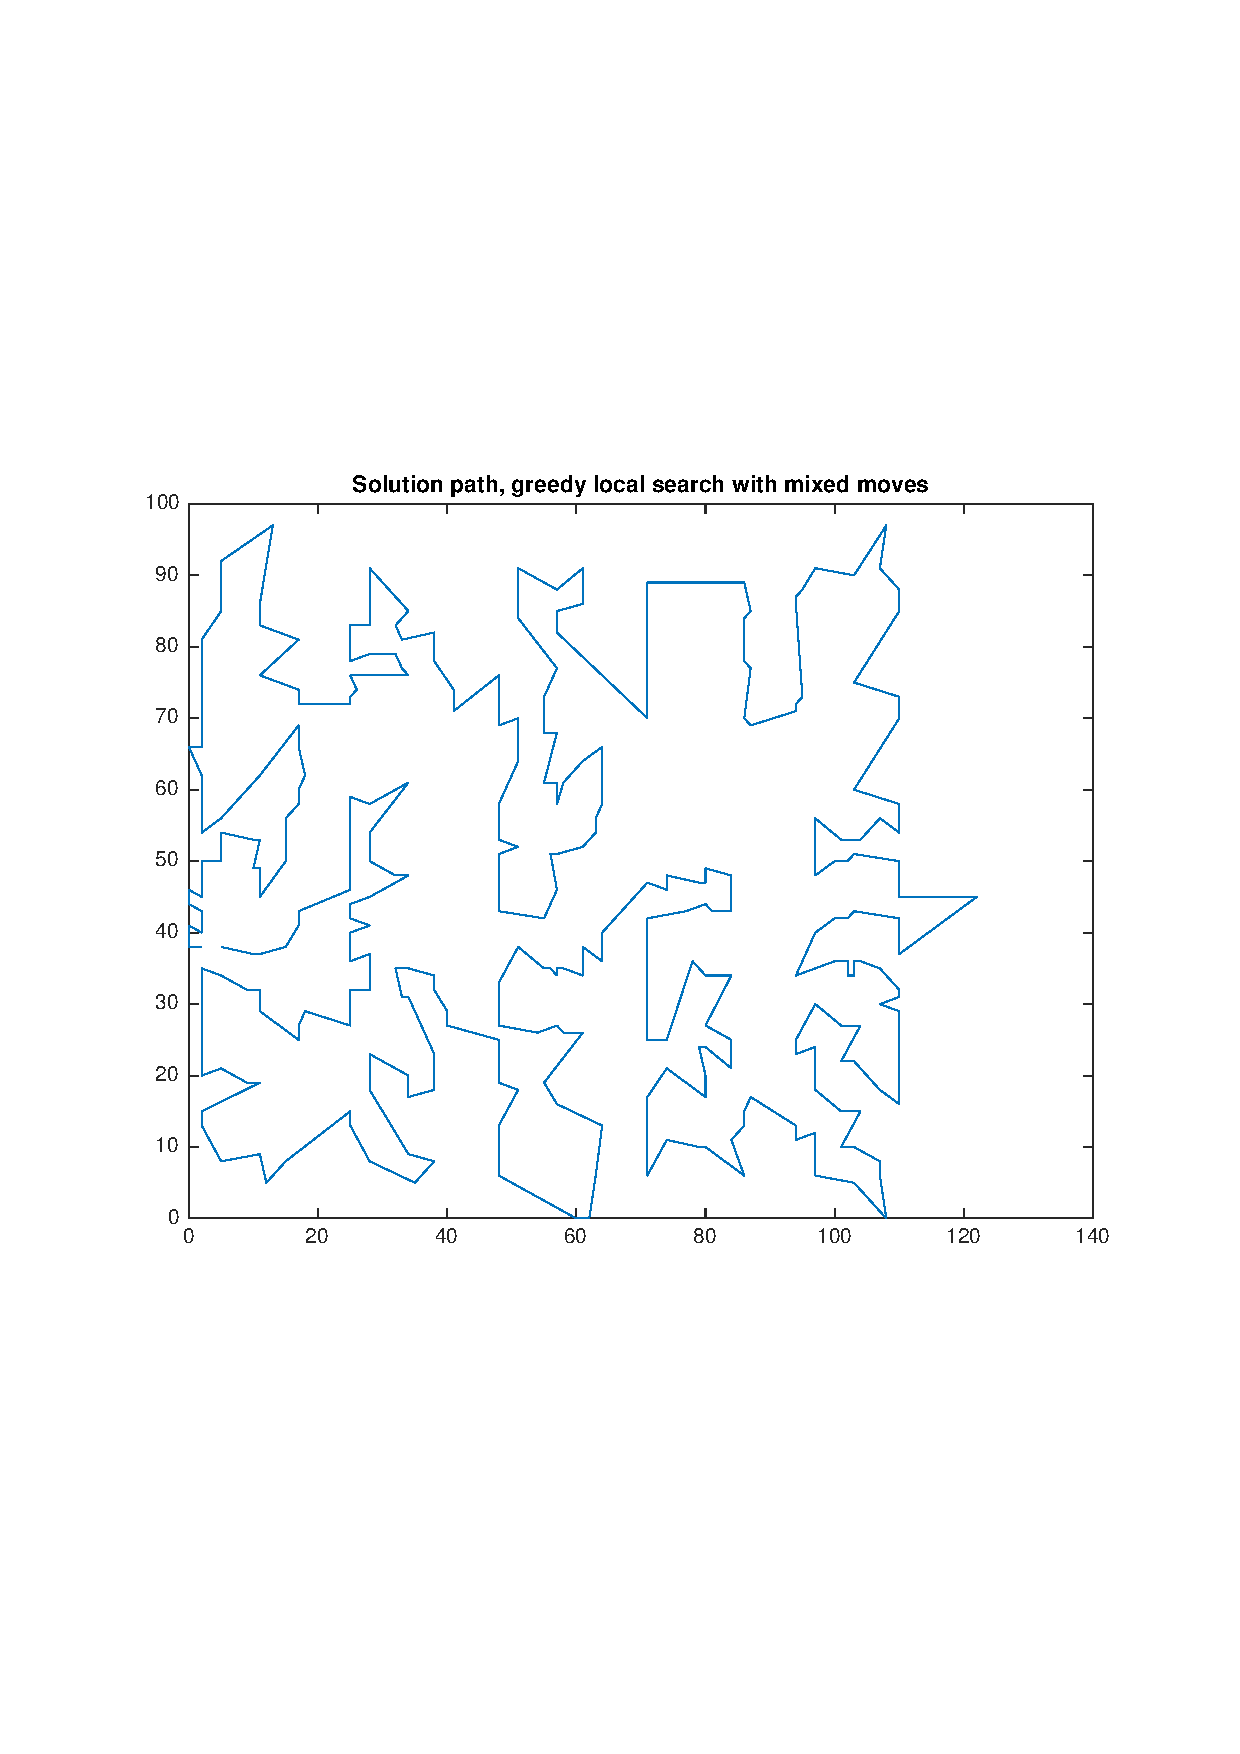
\includegraphics[scale=0.4, trim={3cm 6cm 1cm 6cm}]{../figures/solutionPath_mixed.pdf}
  \end{tabular}
  \caption{Solution path greedy local search heuristics}
  \label{fig:solpath-GLS}
\end{figure}

\begin{figure}[!ht]
  \centering
  \begin{tabular}{cc}
    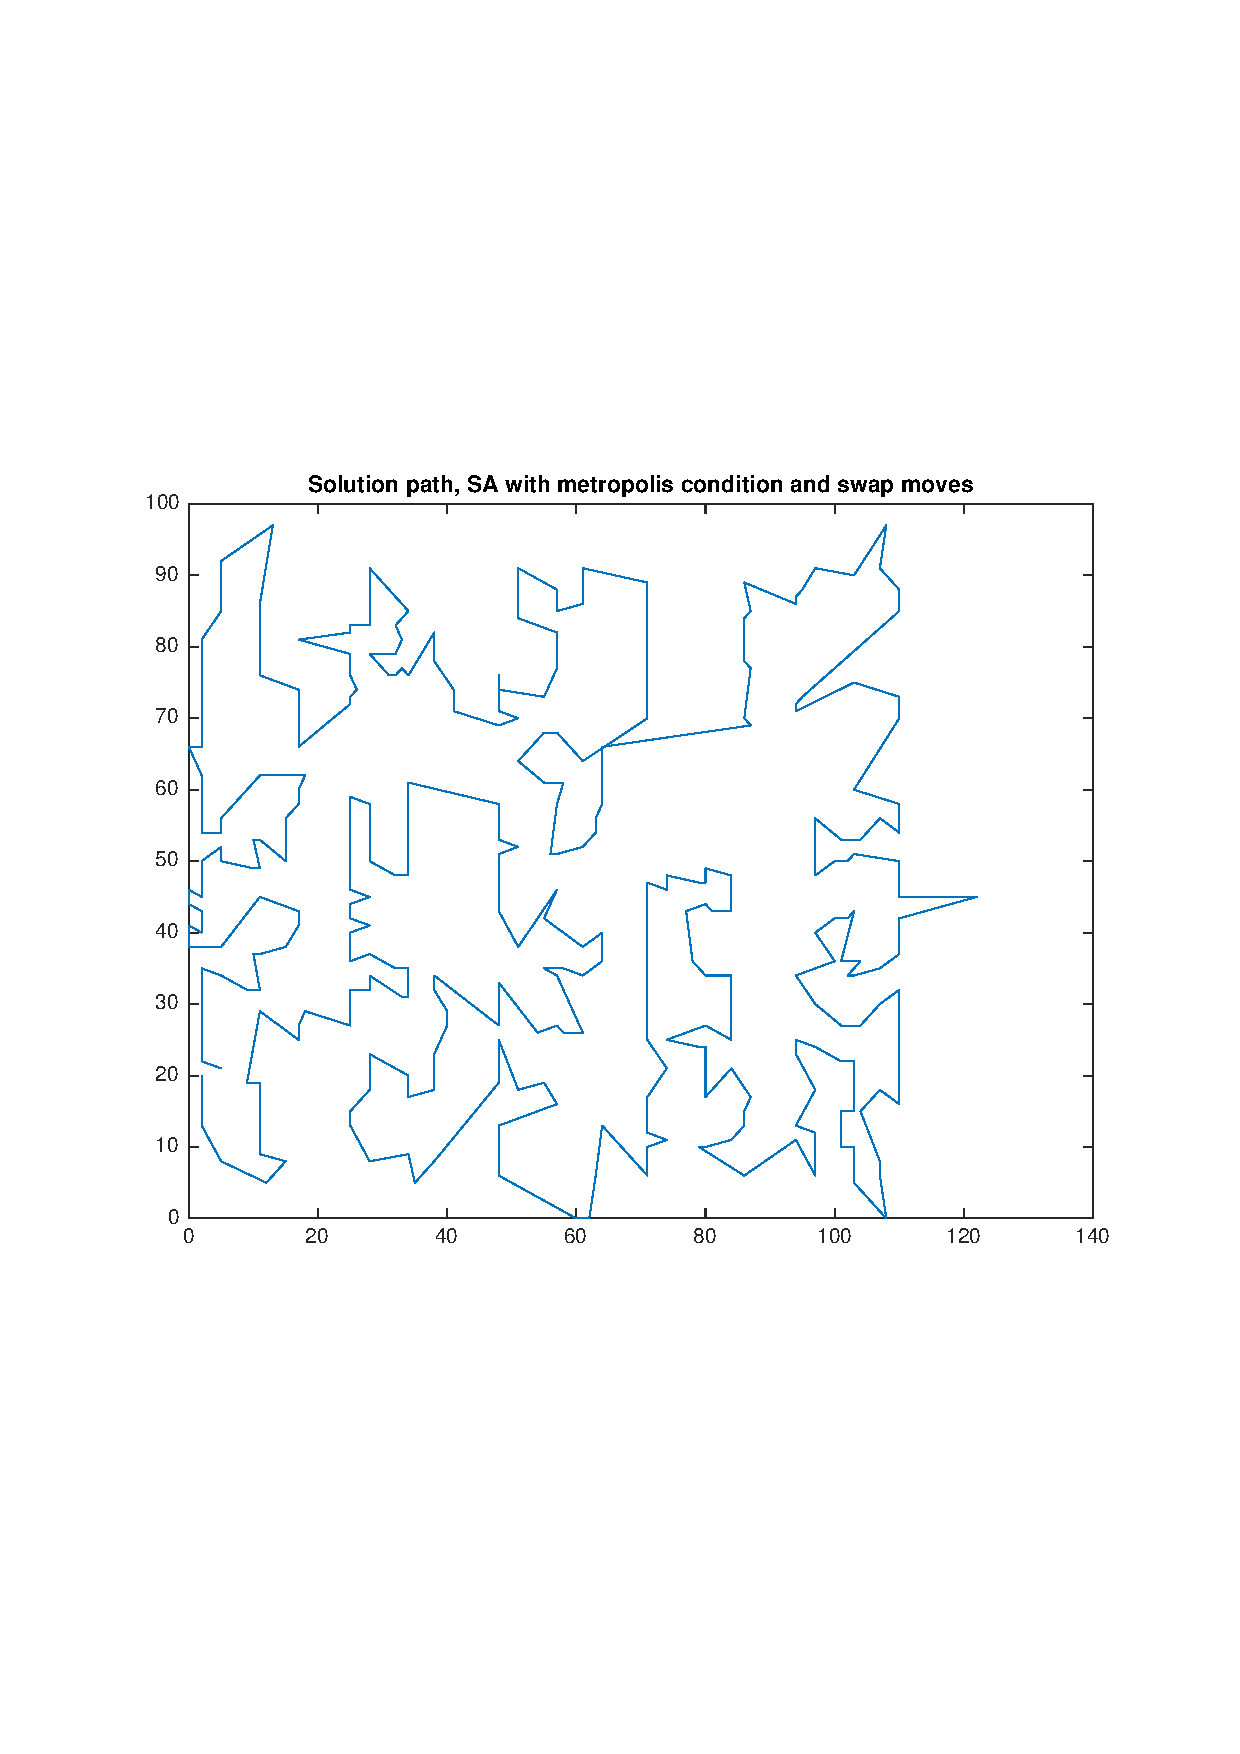
\includegraphics[scale=0.4, trim={3cm 6cm 1cm 6cm}]{../figures/solutionPath_SA_metropolis_swap.pdf} & 
    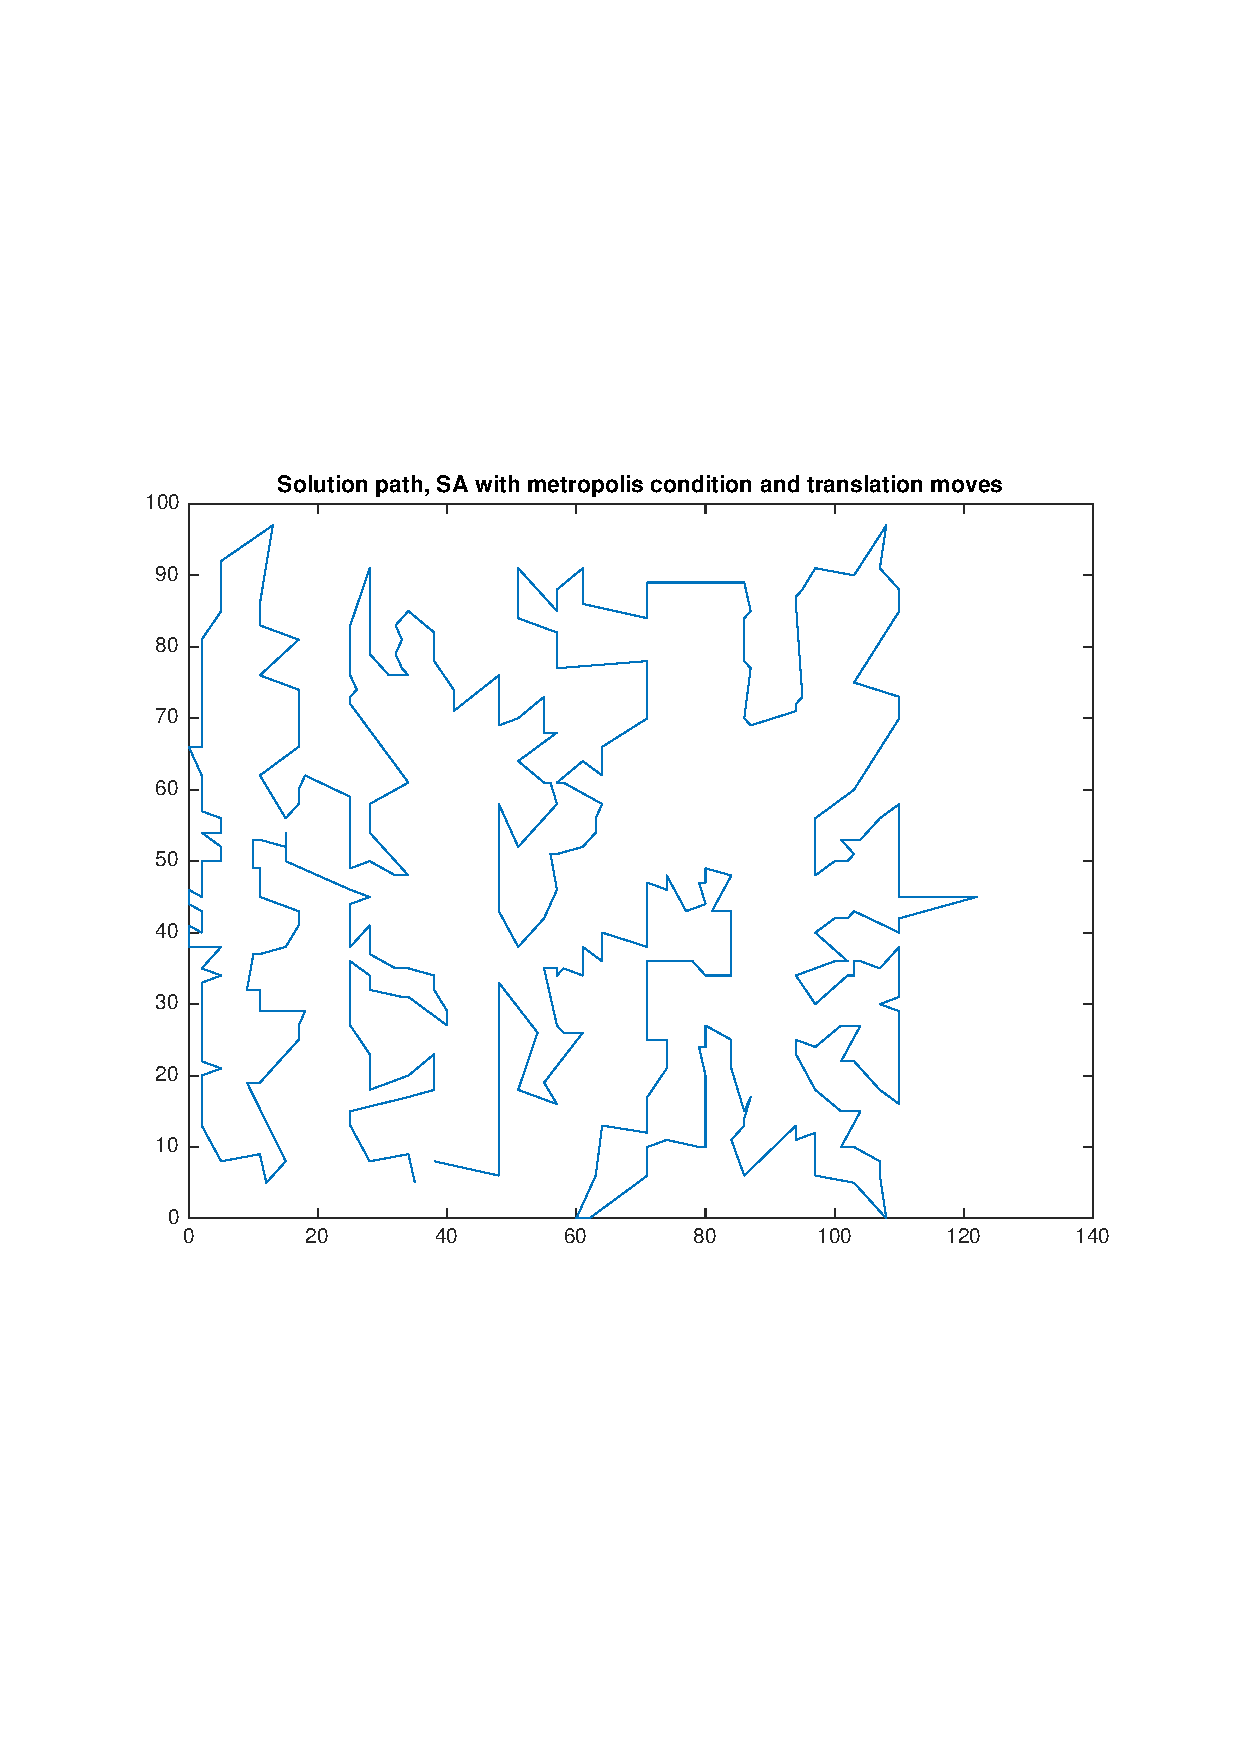
\includegraphics[scale=0.4, trim={3cm 6cm 1cm 6cm}]{../figures/solutionPath_SA_metropolis_translation.pdf} \\ 
    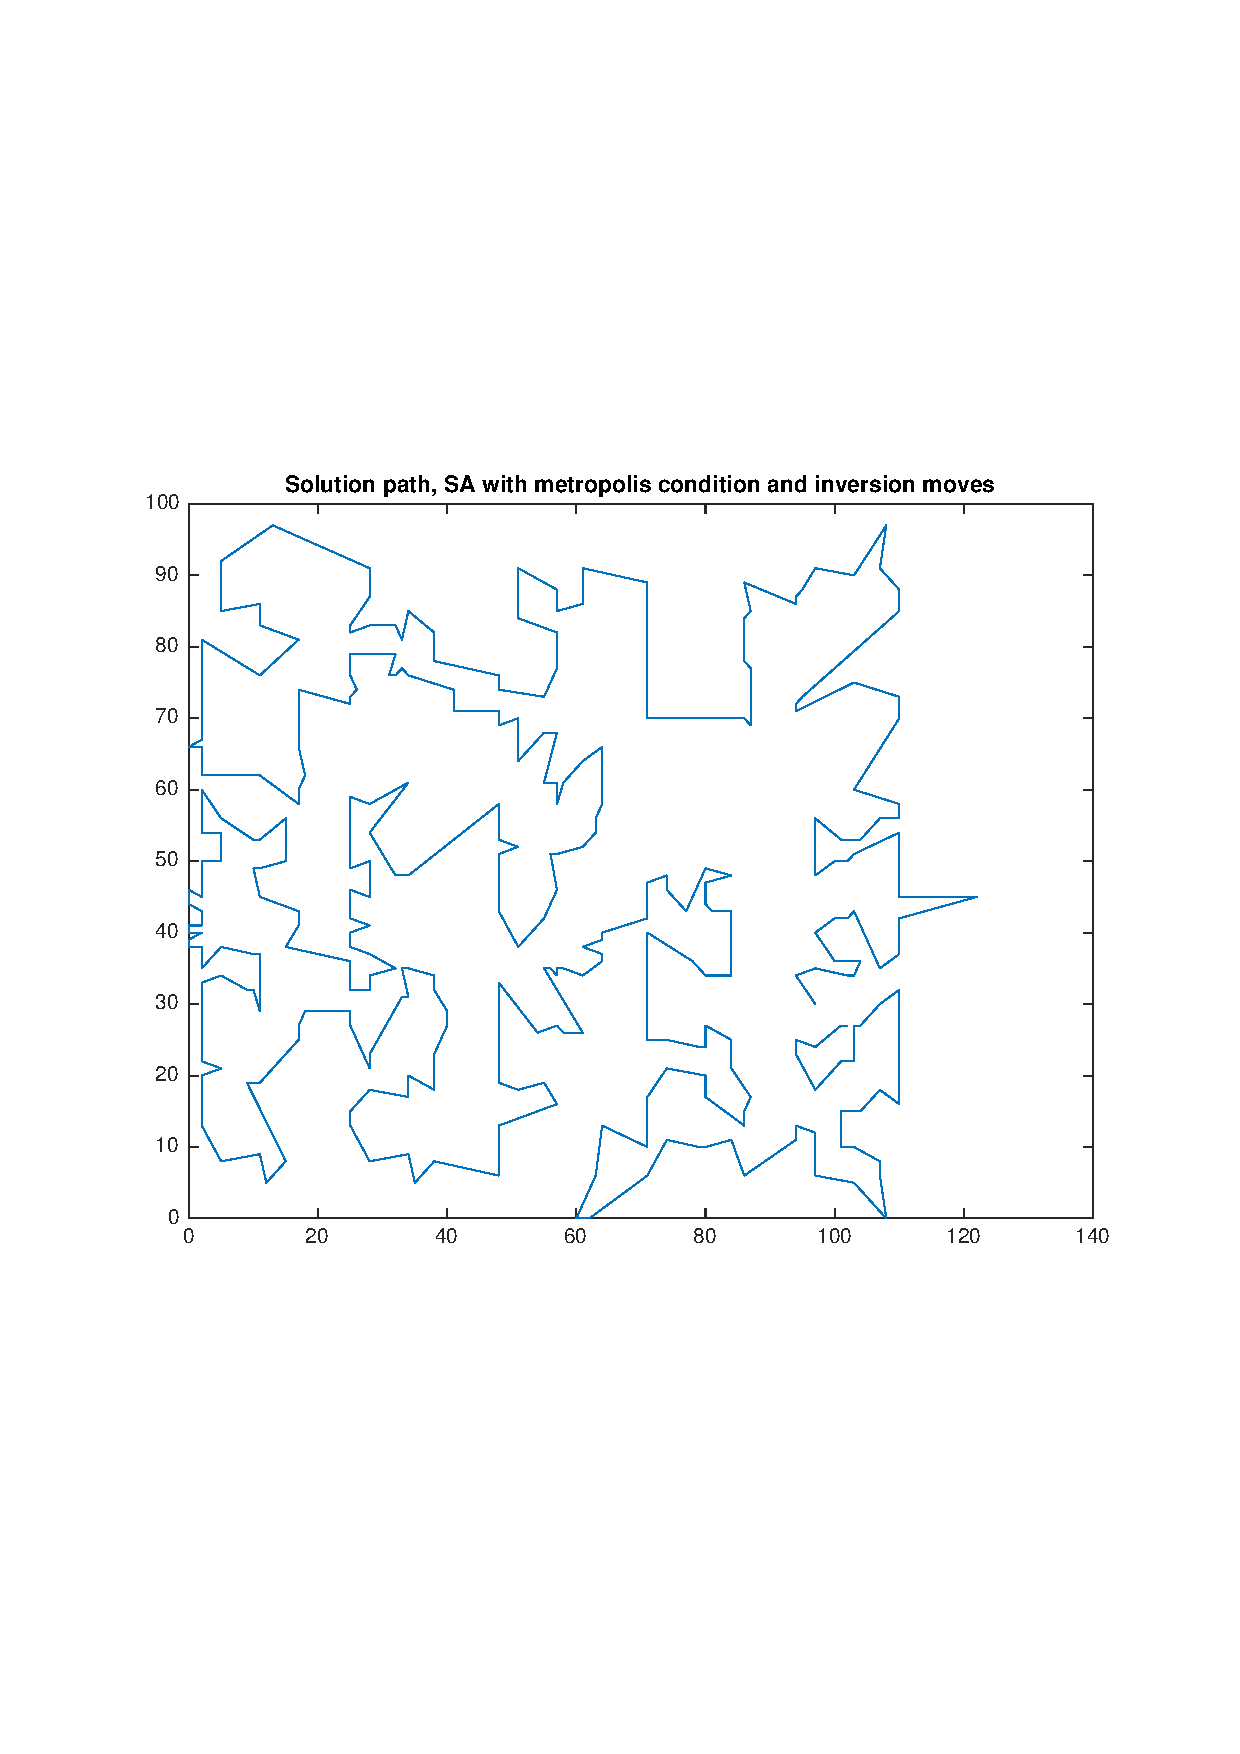
\includegraphics[scale=0.4, trim={3cm 6cm 1cm 6cm}]{../figures/solutionPath_SA_metropolis_inversion.pdf} & 
    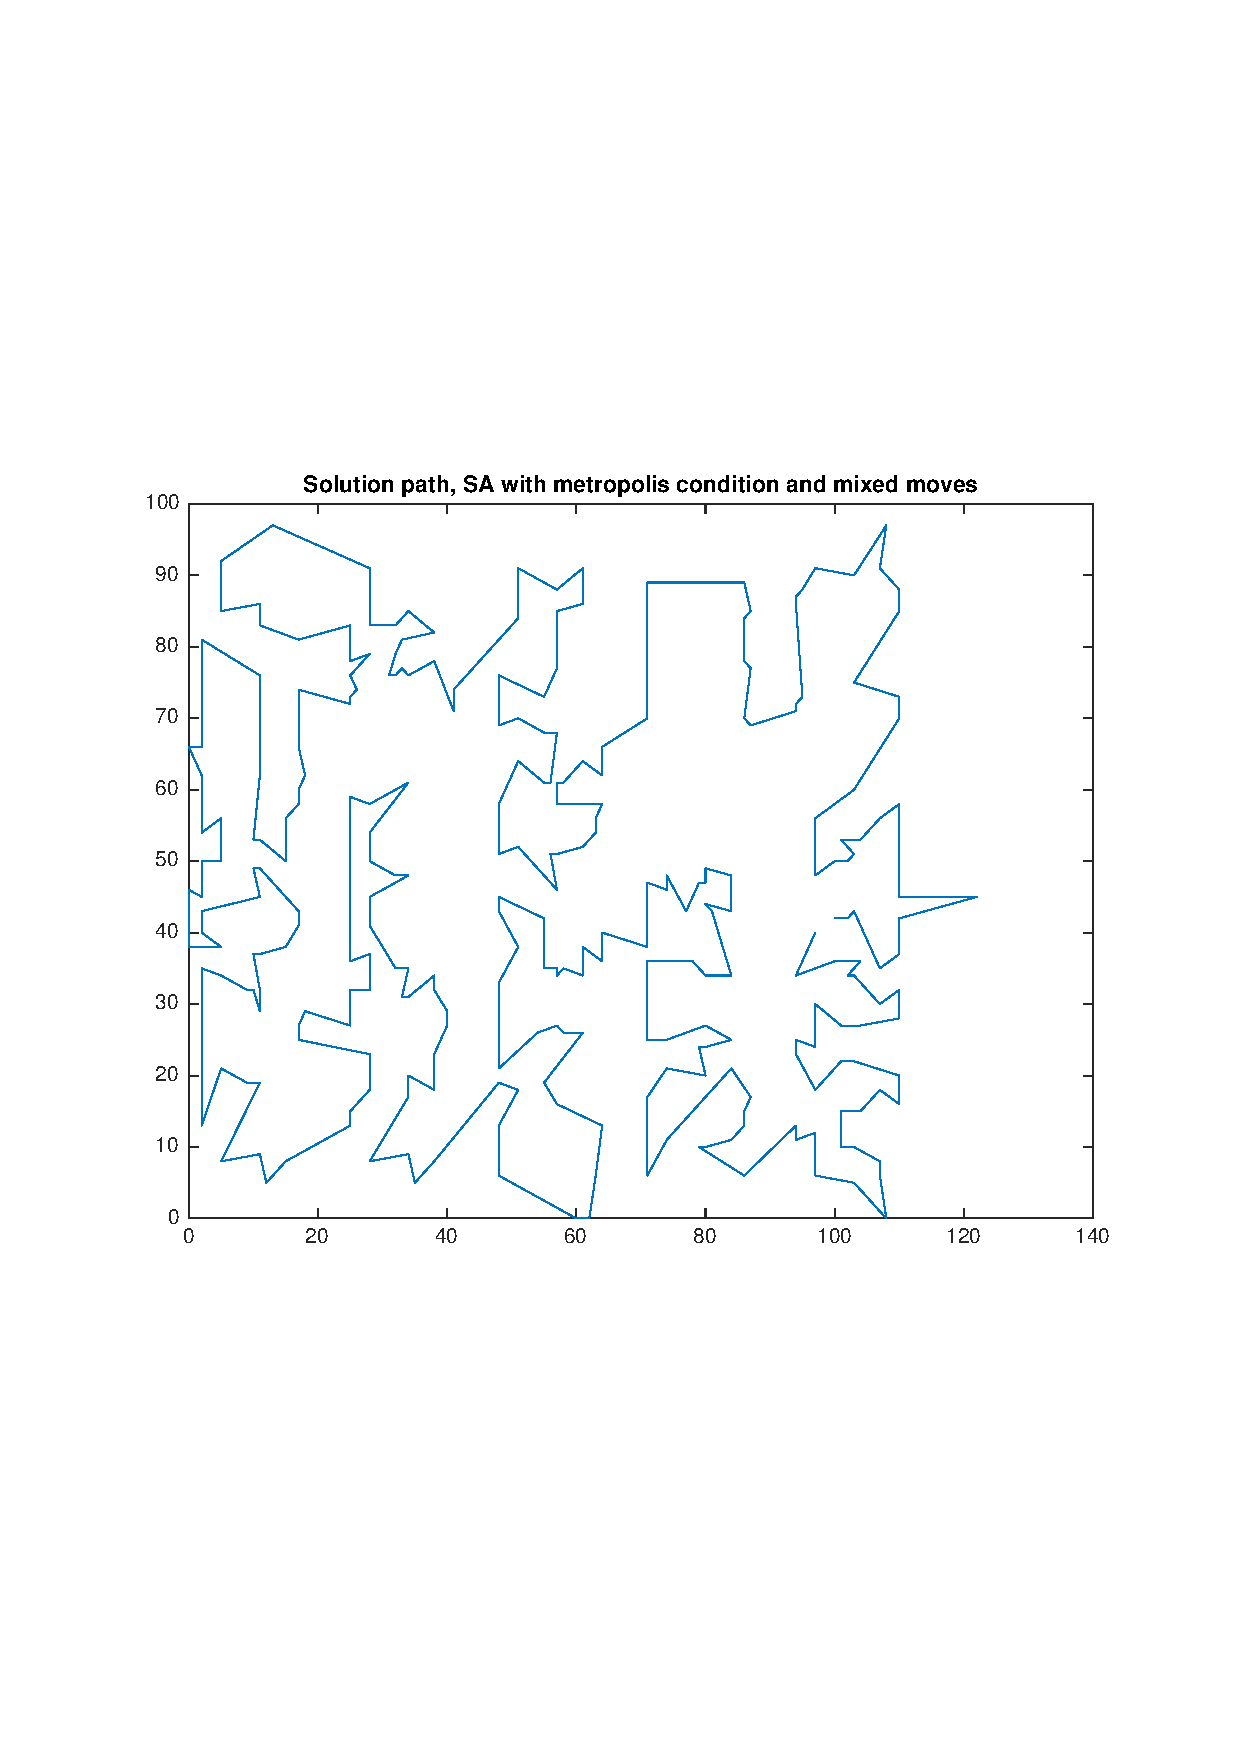
\includegraphics[scale=0.4, trim={3cm 6cm 1cm 6cm}]{../figures/solutionPath_SA_metropolis_mixed.pdf}
  \end{tabular}
  \caption{Solution path SA algorithm with metropolis criterion}
  \label{fig:solpath-SA-metropolis}
\end{figure}

\begin{figure}[!ht]
  \centering
  \begin{tabular}{cc}
    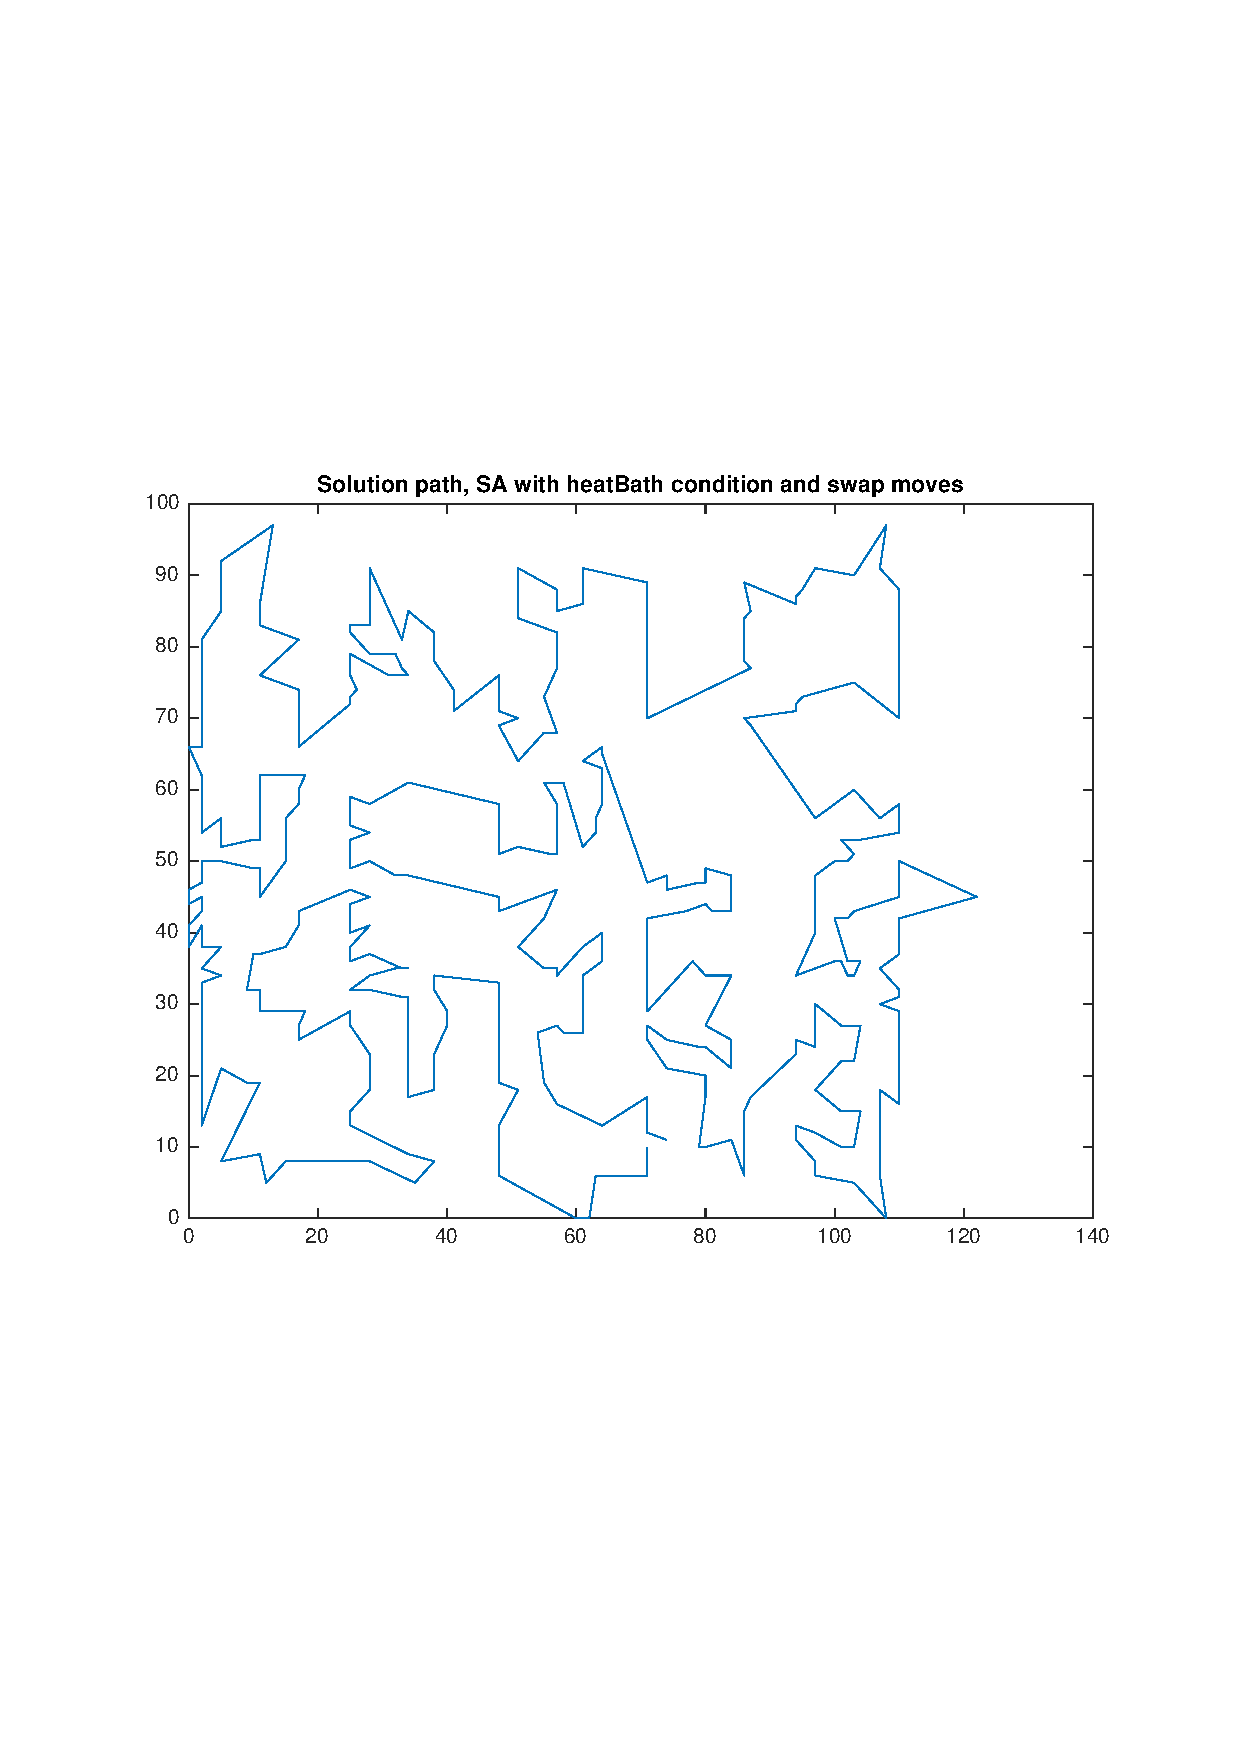
\includegraphics[scale=0.4, trim={3cm 6cm 1cm 6cm}]{../figures/solutionPath_SA_heatBath_swap.pdf} & 
    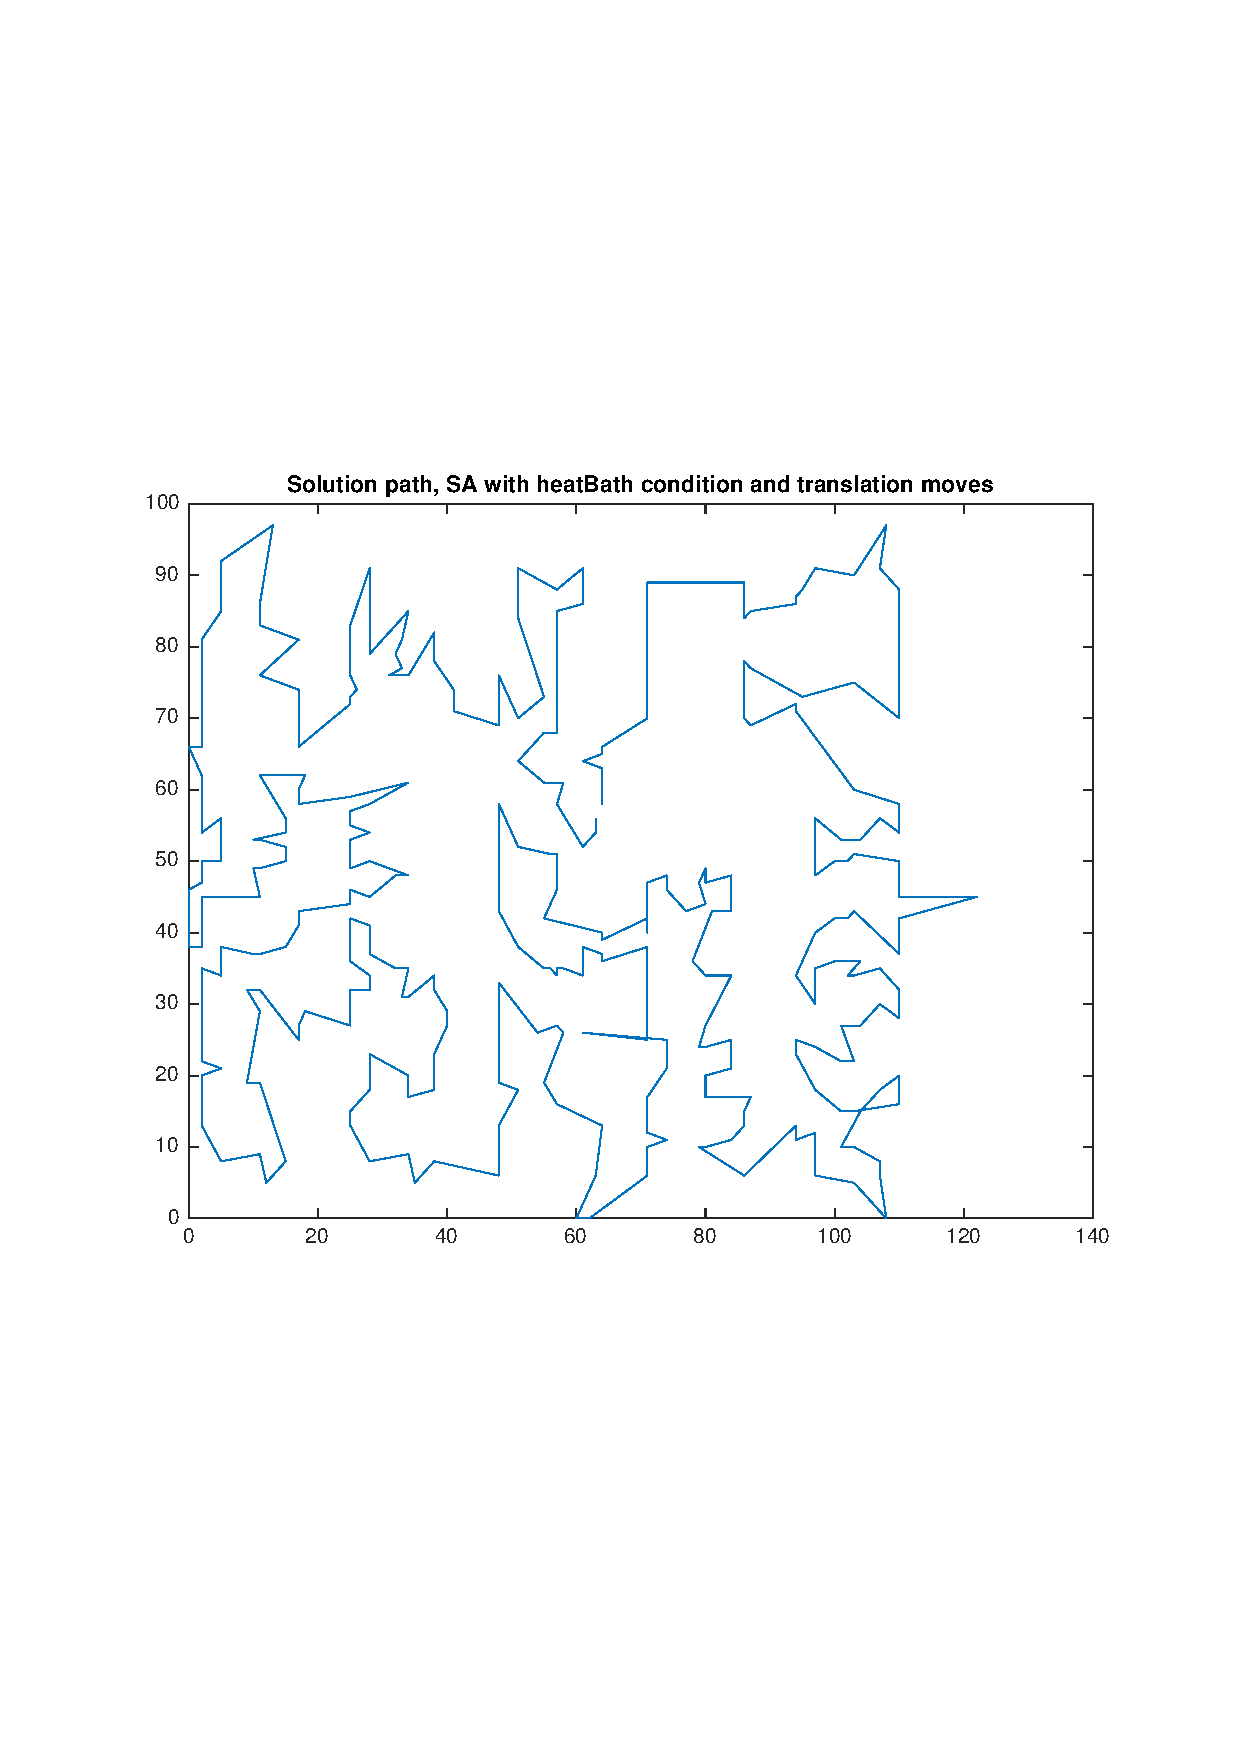
\includegraphics[scale=0.4, trim={3cm 6cm 1cm 6cm}]{../figures/solutionPath_SA_heatBath_translation.pdf} \\ 
    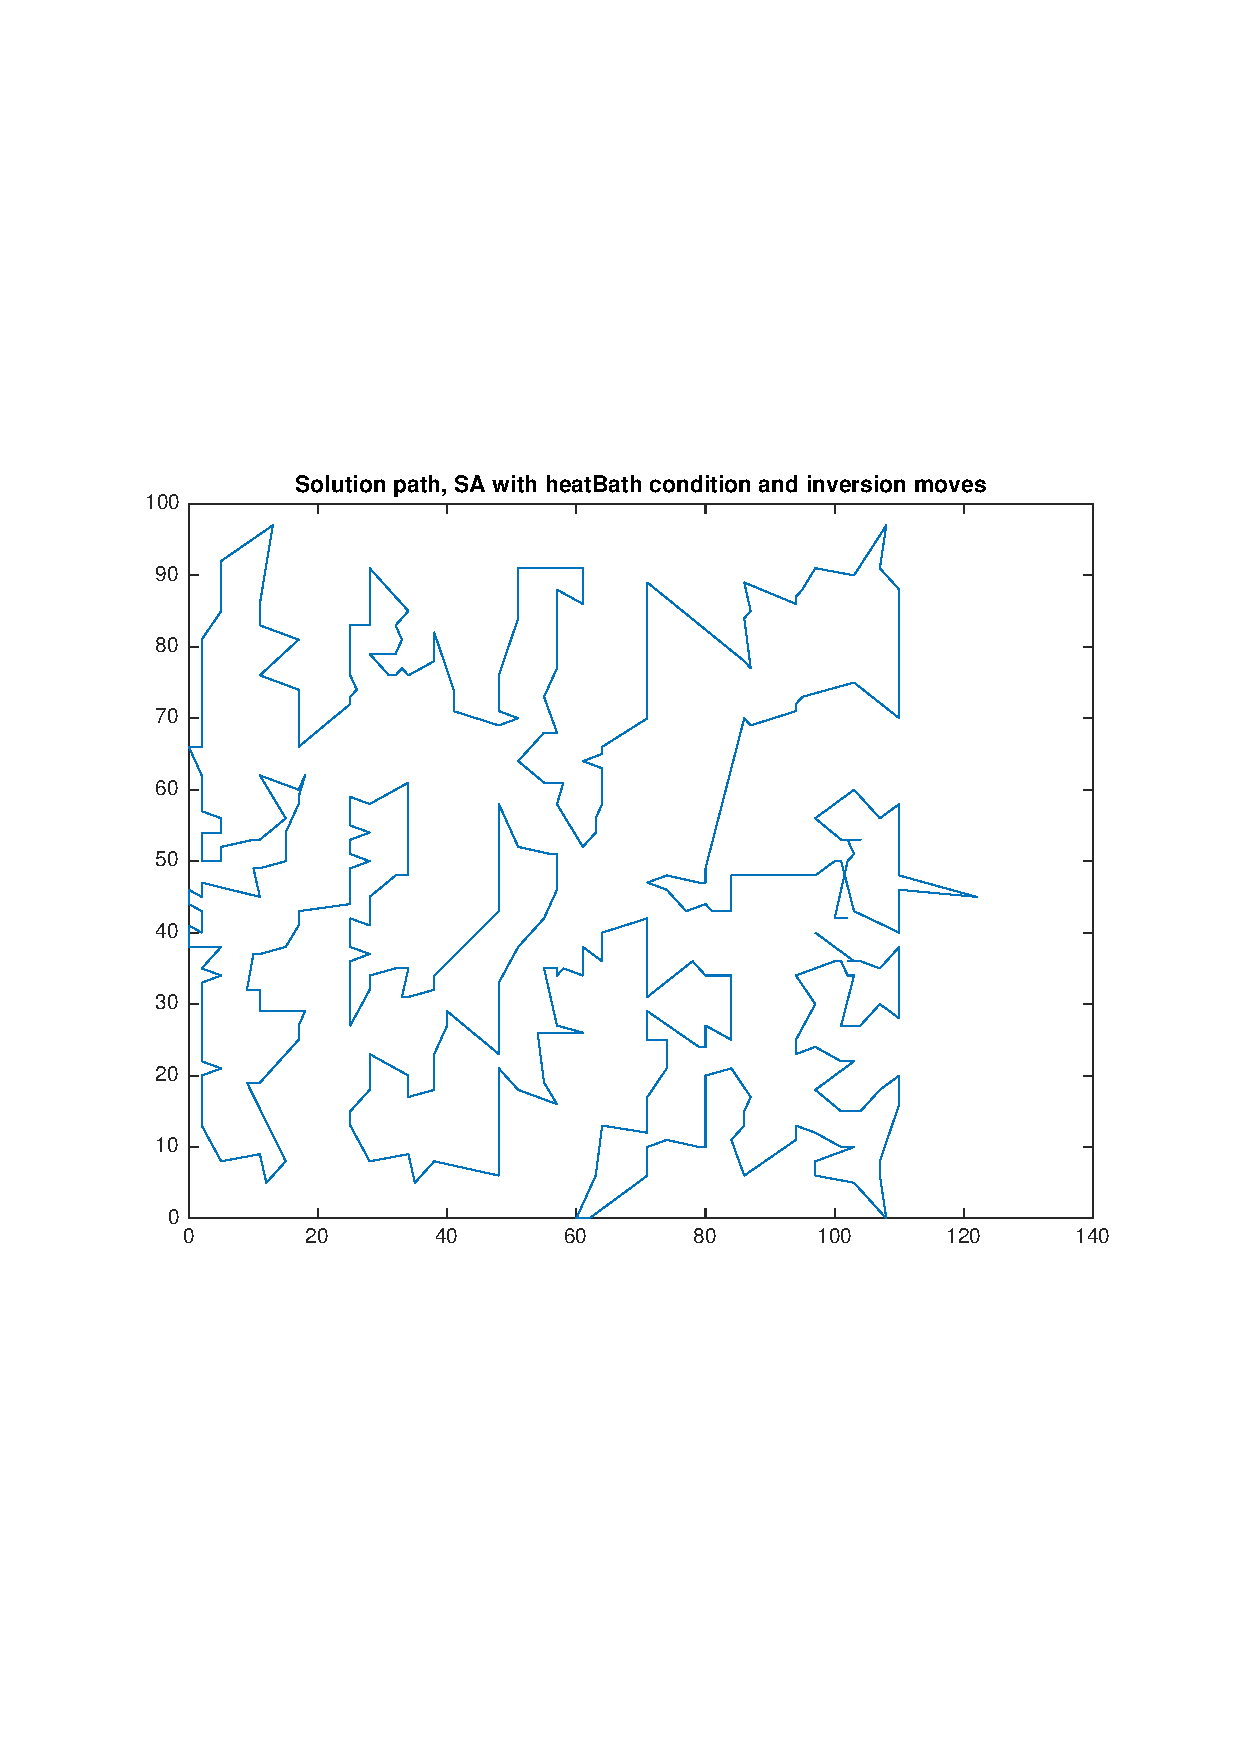
\includegraphics[scale=0.4, trim={3cm 6cm 1cm 6cm}]{../figures/solutionPath_SA_heatBath_inversion.pdf} & 
    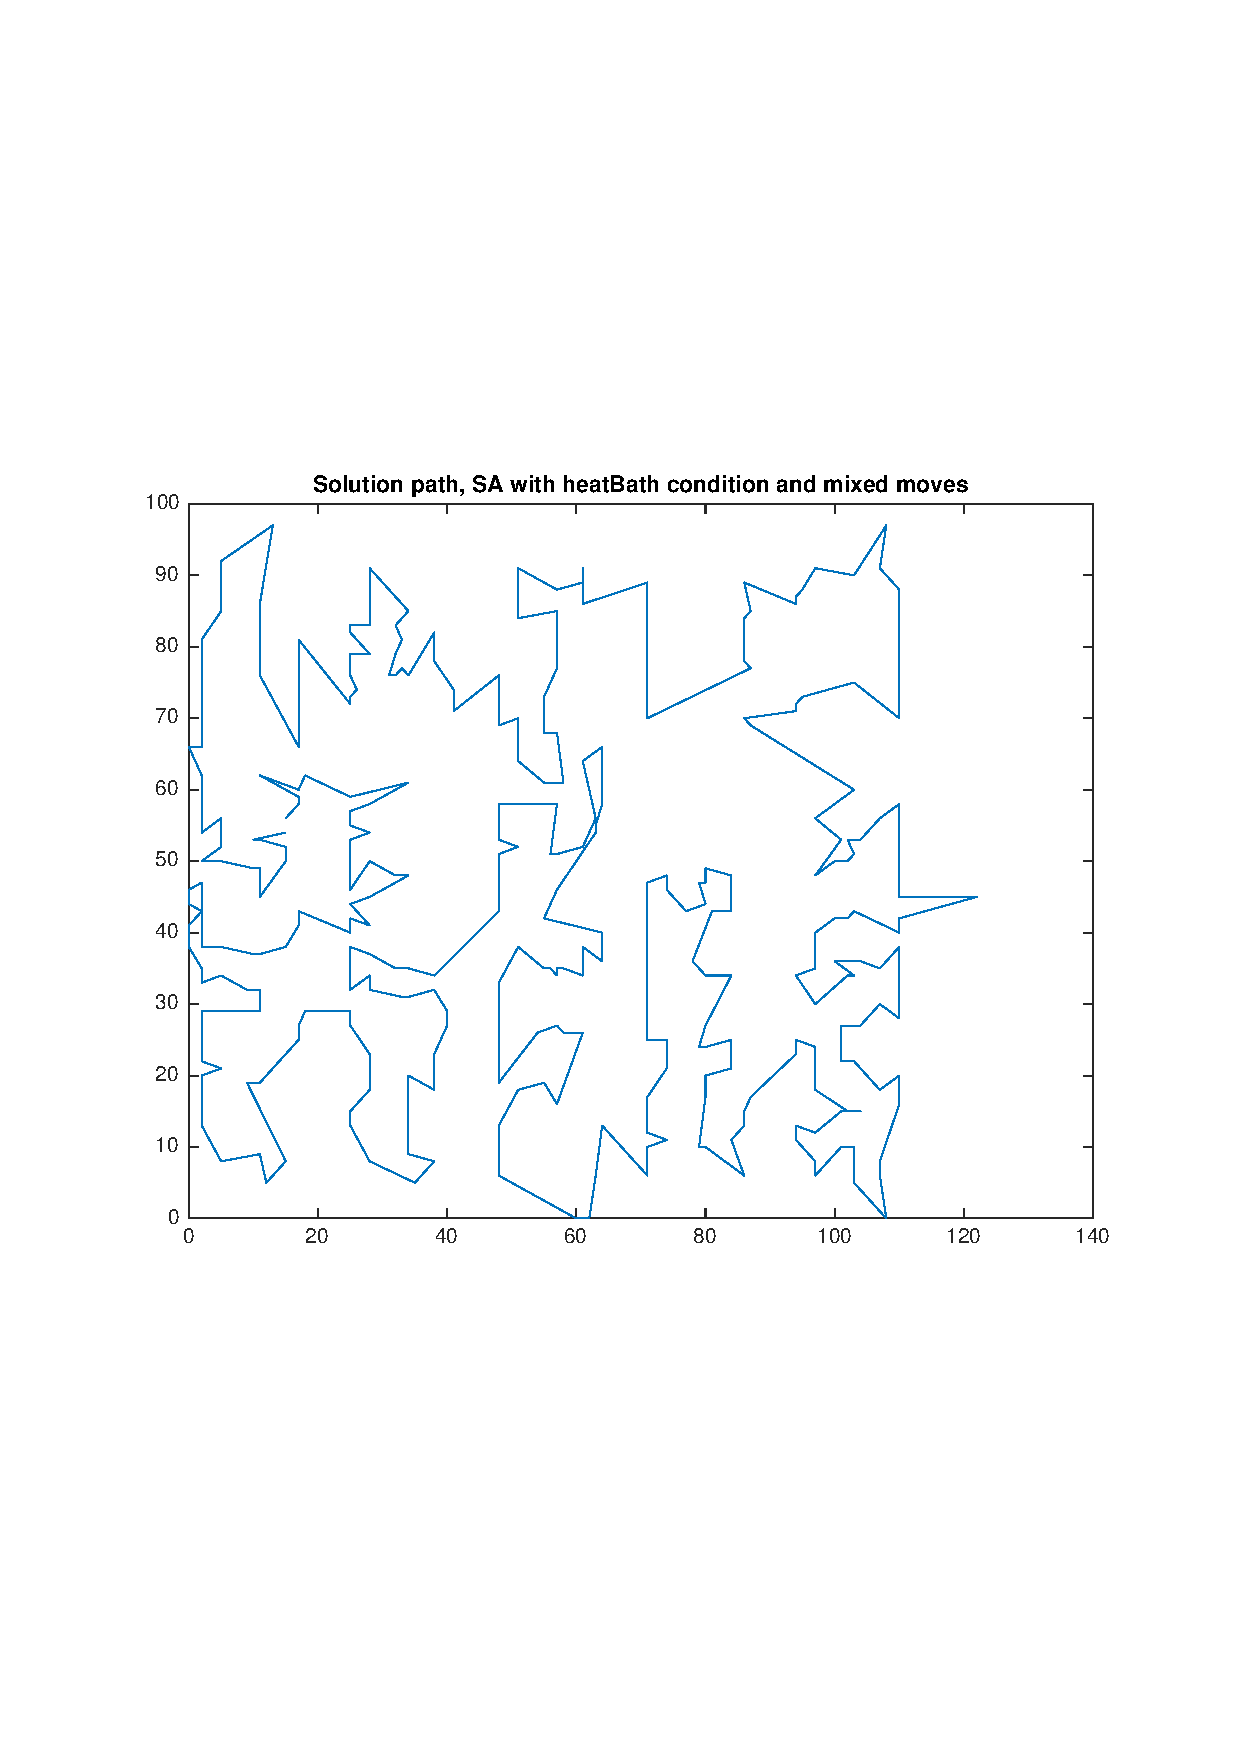
\includegraphics[scale=0.4, trim={3cm 6cm 1cm 6cm}]{../figures/solutionPath_SA_heatBath_mixed.pdf}
  \end{tabular}
  \caption{Solution path SA algorithm with heat bath criterion}
  \label{fig:solpath-SA-heatBath}
\end{figure}

We show the trace of the best tour found after 30 rounds of each algorithms. For the improvement algorithms
and the SA algorithm, the first tour is constructed with the best insertion algorithm. The traces are shown in
Figures \ref{fig:solpath-bestinsertion} to \ref{fig:solpath-SA-heatBath}.



\section{Performance plots}
\label{sec:performance-plots}

We now present the performance plots, which show the evolution of the path length over the different
iterations. For the greedy local search, the path length is represented as a function of the number of steps
of the algorithms, and for the simulated annealing algorithms, the path length is a function of the
temperature. The performance plots are represented in Figures \ref{fig:perfPlot-GLS} to
\ref{fig:perfPlot-SA-heatBath}.

On plot \ref{fig:perfPlot-GLS}, we see that for each of the small moves, the gain in path length is not that
huge, but the translation and inversion moves seem to give better results than the swap move. The biggest gain
is obtained by using the mixed moves, as we saw in Section 2.

On the other hand, for the SA algorithm, due to the fact that the temperature is very hot at the beginning, we
accept worse solutions, with a big path length, but the path length decreases very fast near its optimal
value. The best result seem to be achieved when using the inversion small moves, as the stopping condition is
met when the temperature is almost $10^{10}$ times bigger, which is a huge improvement. In this case, using
translations as small moves seems to be the worst case, as we need to decrease the temperature a lot before
meeting the stopping criterion. 

If we use the metropolis criterion, using mixed small moves seems to be a good idea, as the result are not so
bad, and mixed moves are versatile. When using the heat bath condition, the mixed moves are not the best
choice, but this may come from an unlucky run. 

\begin{figure}[!ht]
  \centering
  \begin{tabular}{cc}
    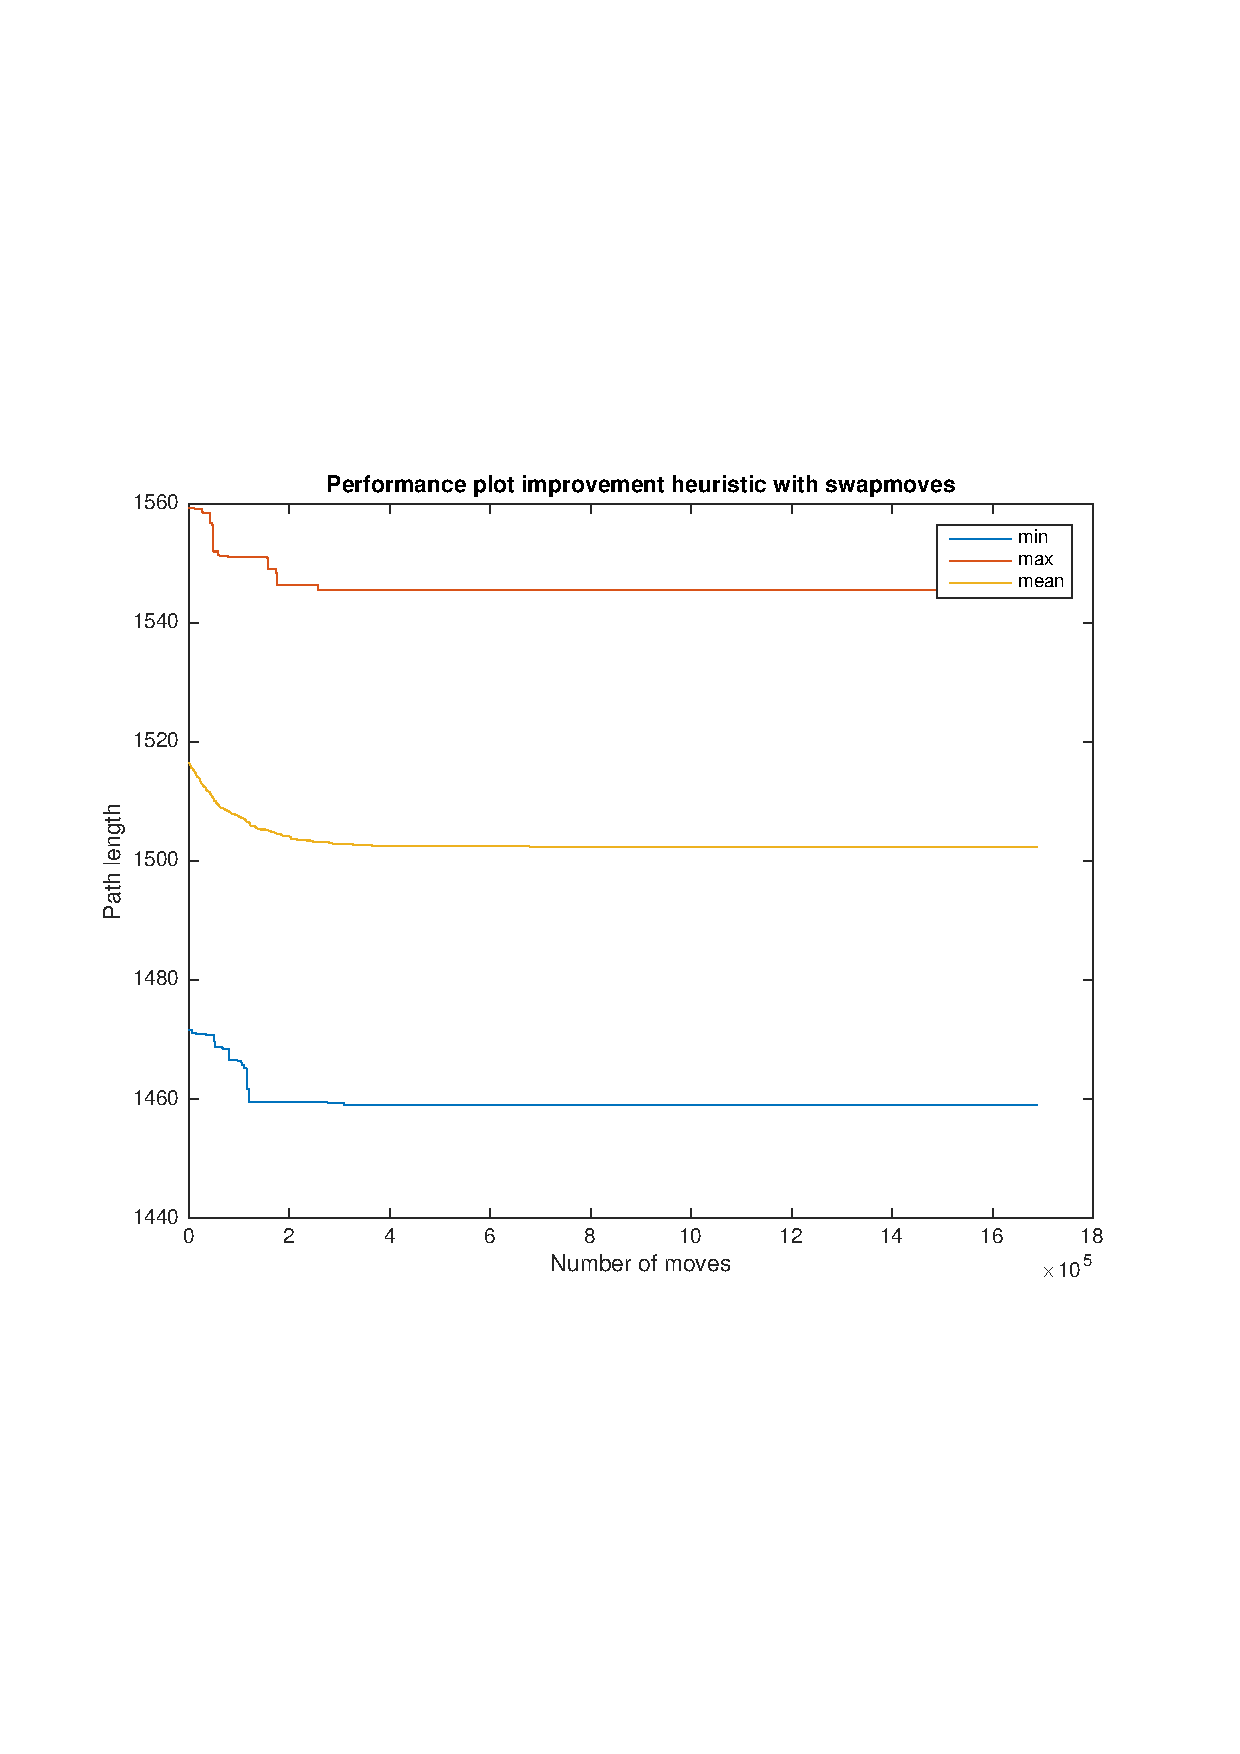
\includegraphics[scale=0.4, trim={3cm 6cm 1cm 6cm}]{../figures/perfPlot_swap.pdf} & 
    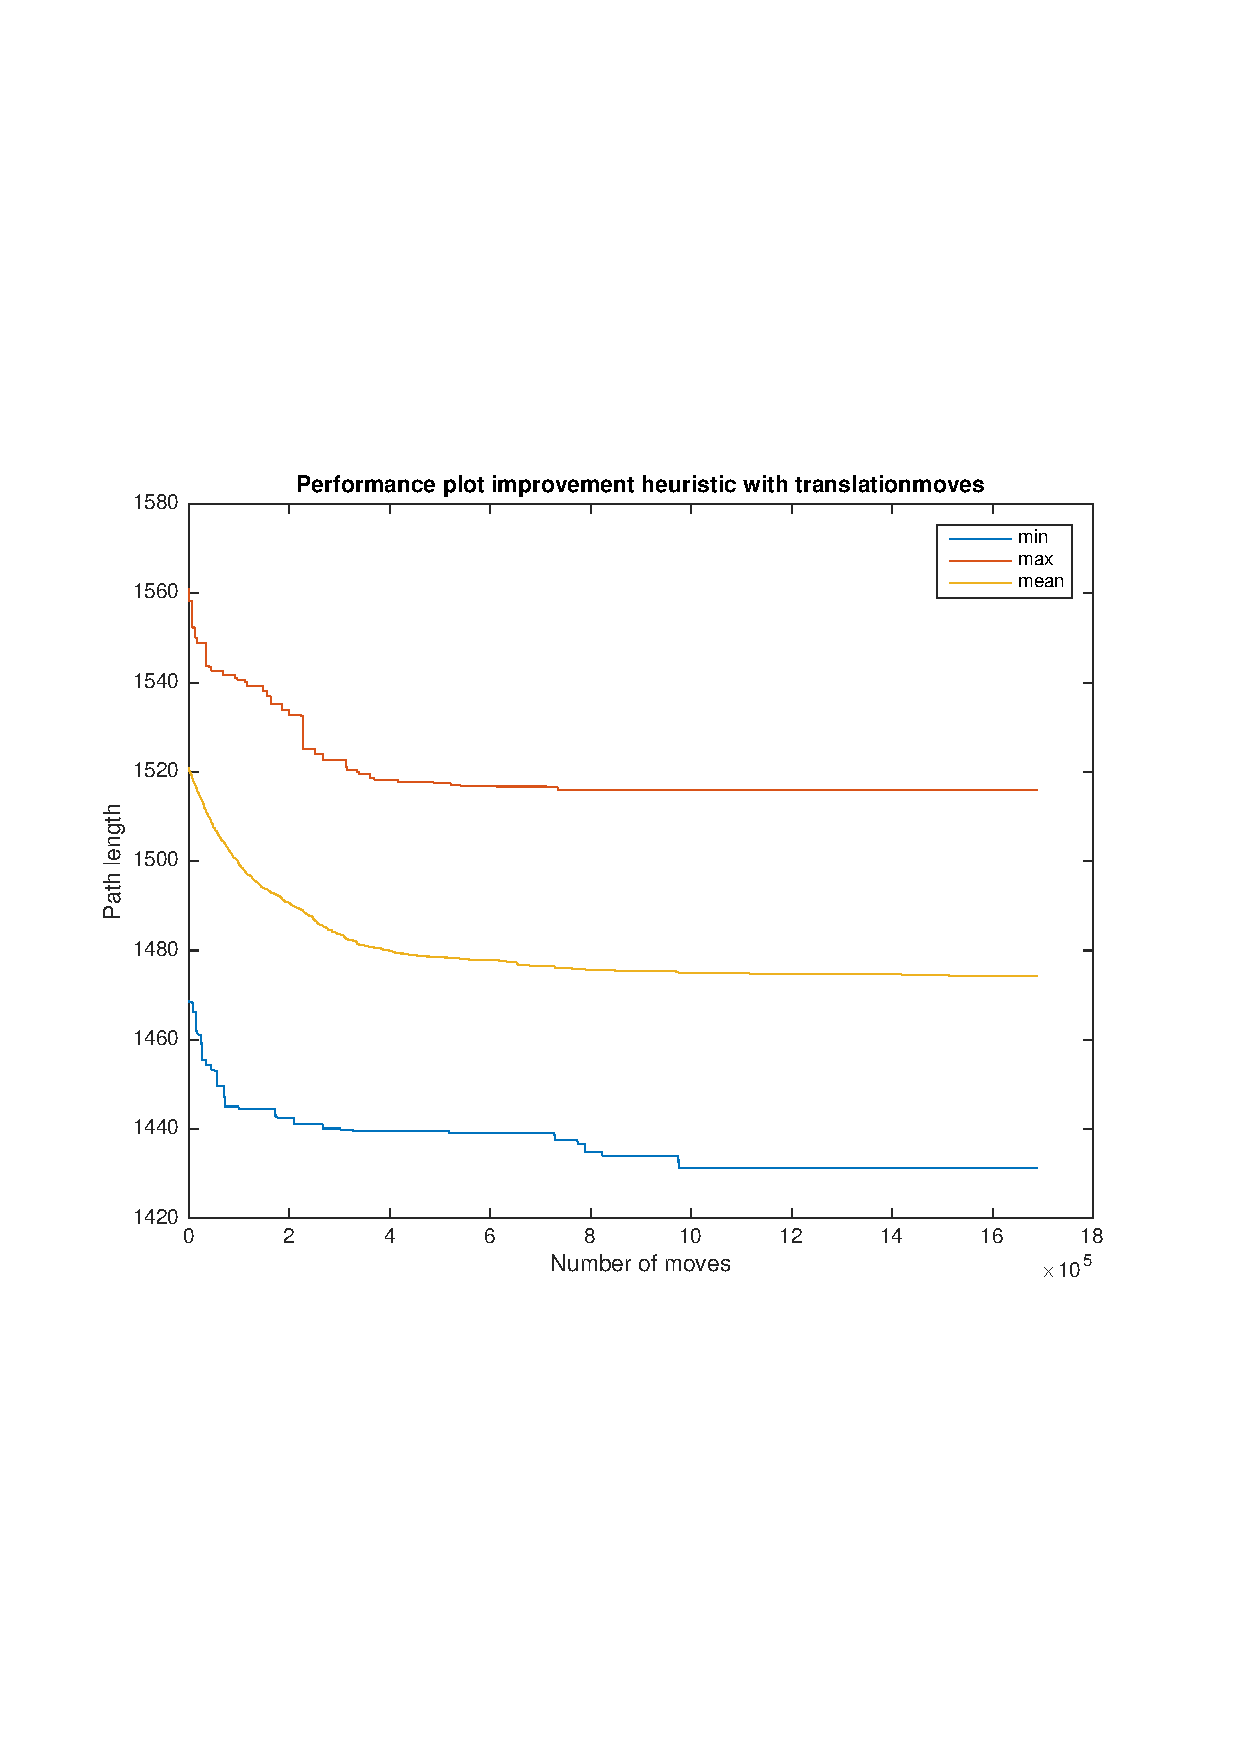
\includegraphics[scale=0.4, trim={3cm 6cm 1cm 6cm}]{../figures/perfPlot_translation.pdf} \\ 
    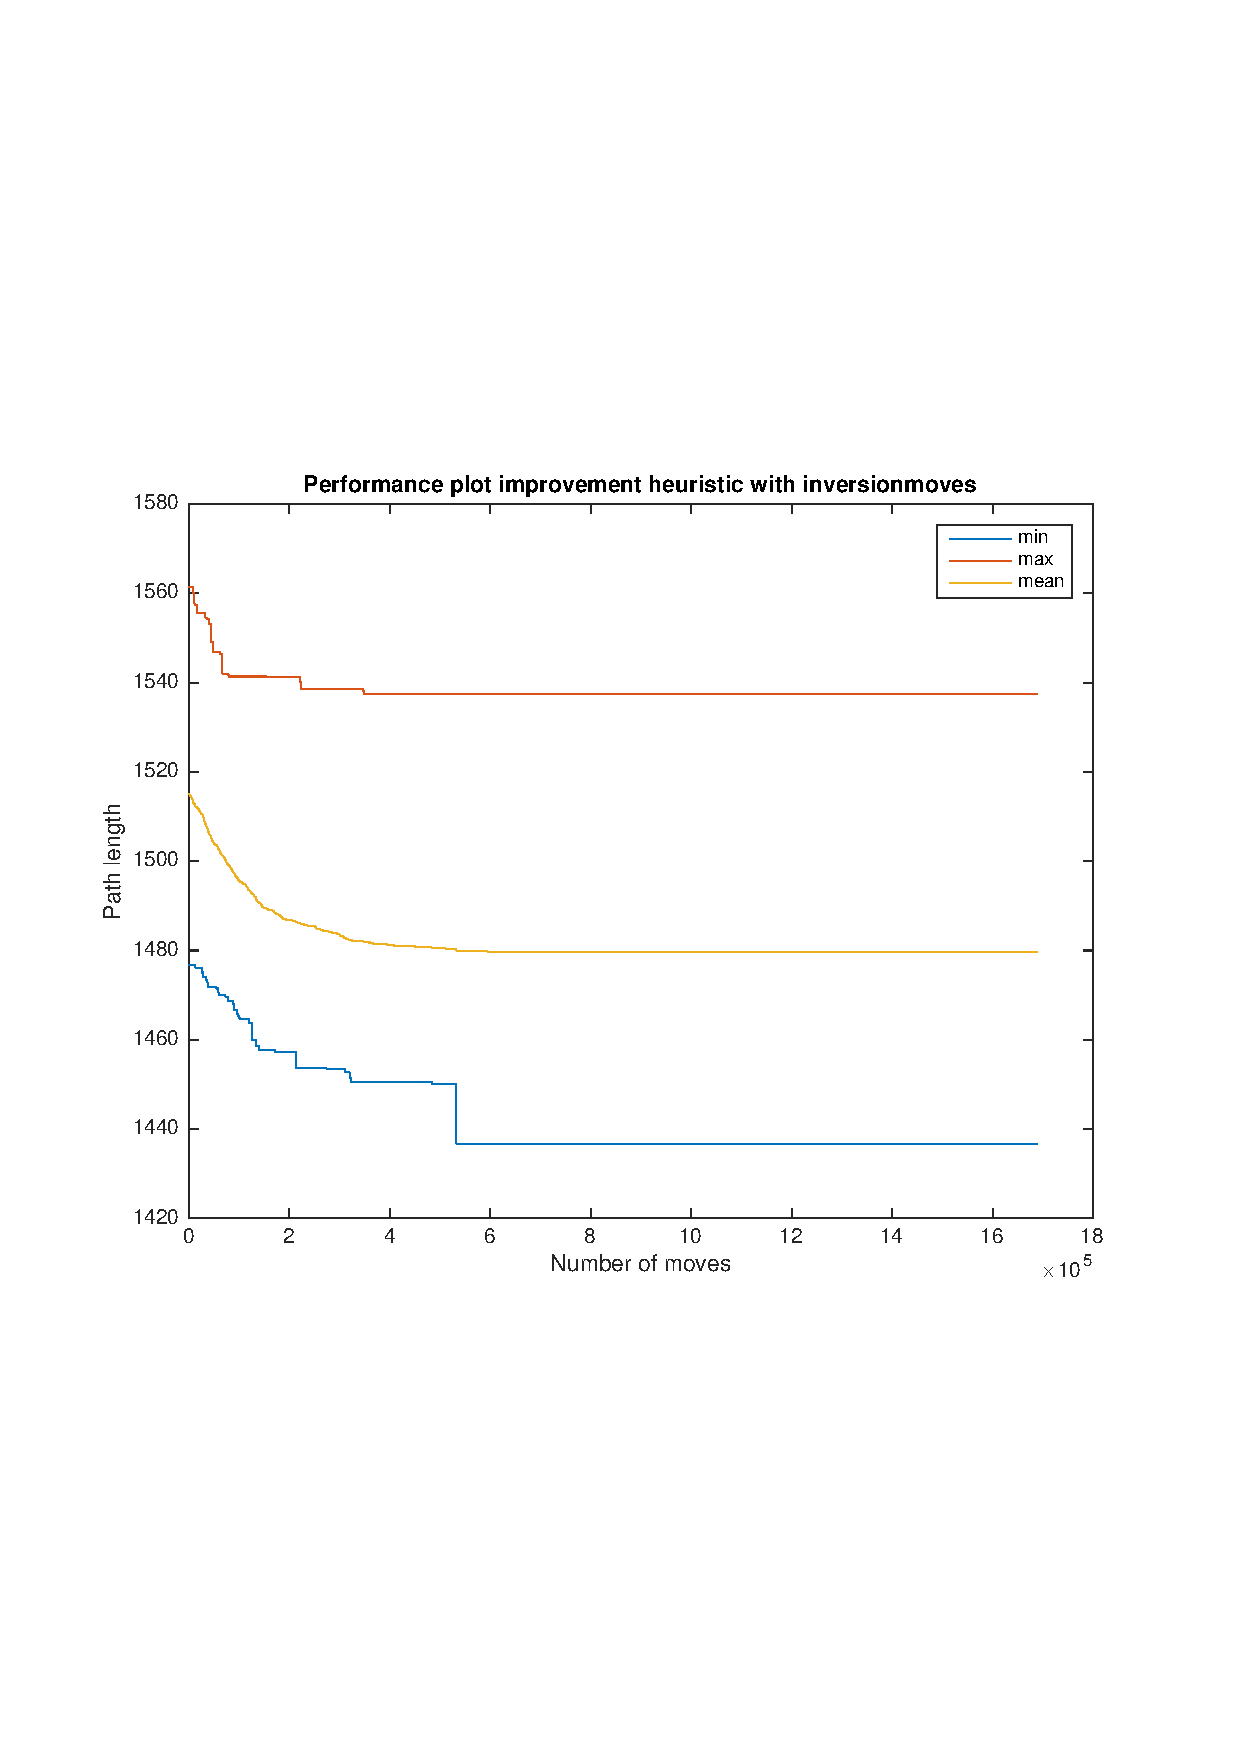
\includegraphics[scale=0.4, trim={3cm 6cm 1cm 6cm}]{../figures/perfPlot_inversion.pdf} & 
    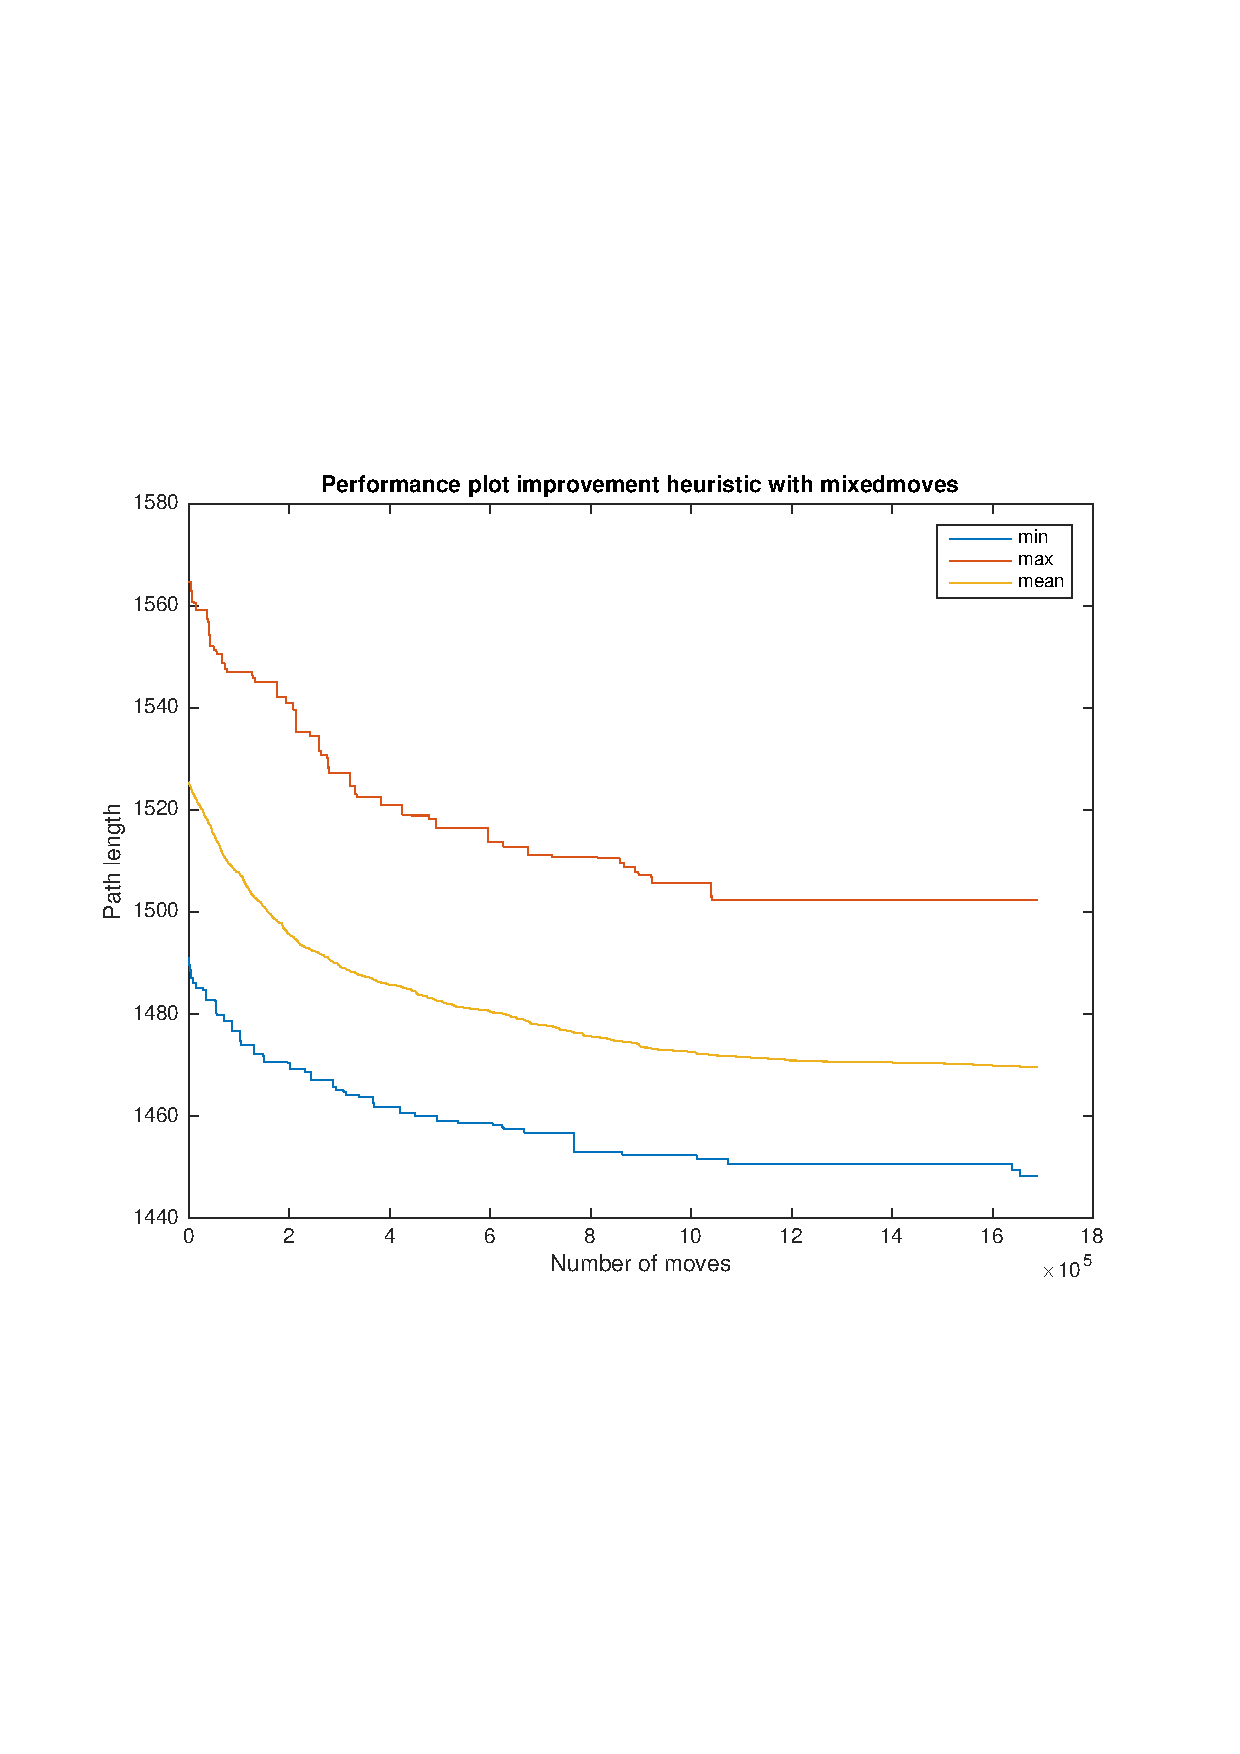
\includegraphics[scale=0.4, trim={3cm 6cm 1cm 6cm}]{../figures/perfPlot_mixed.pdf}
  \end{tabular}
  \caption{Performance plots for the greedy local search}
  \label{fig:perfPlot-GLS}
\end{figure}

\begin{figure}[!ht]
  \centering
  \begin{tabular}{cc}
    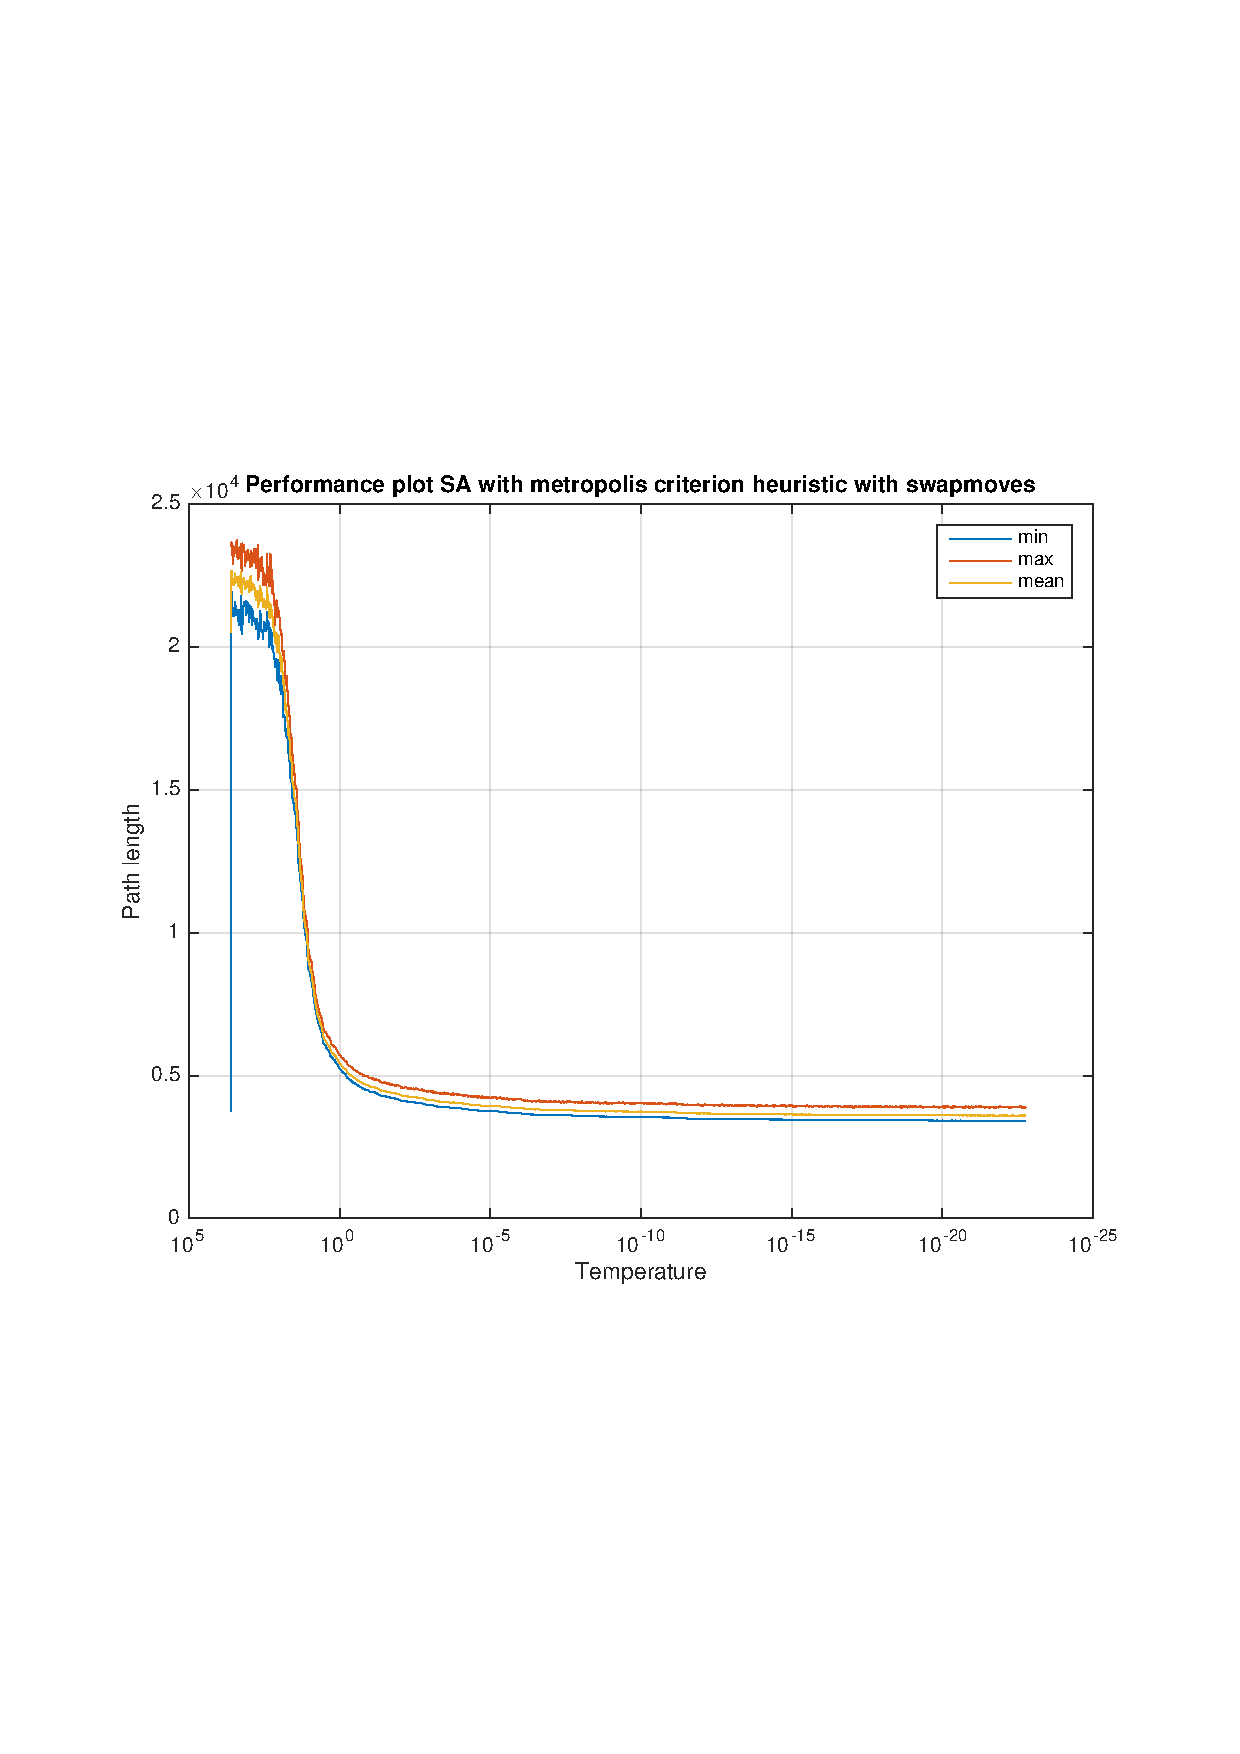
\includegraphics[scale=0.4, trim={3cm 6cm 1cm 6cm}]{../figures/perfPlot_SA_metropolis_swap.pdf} & 
    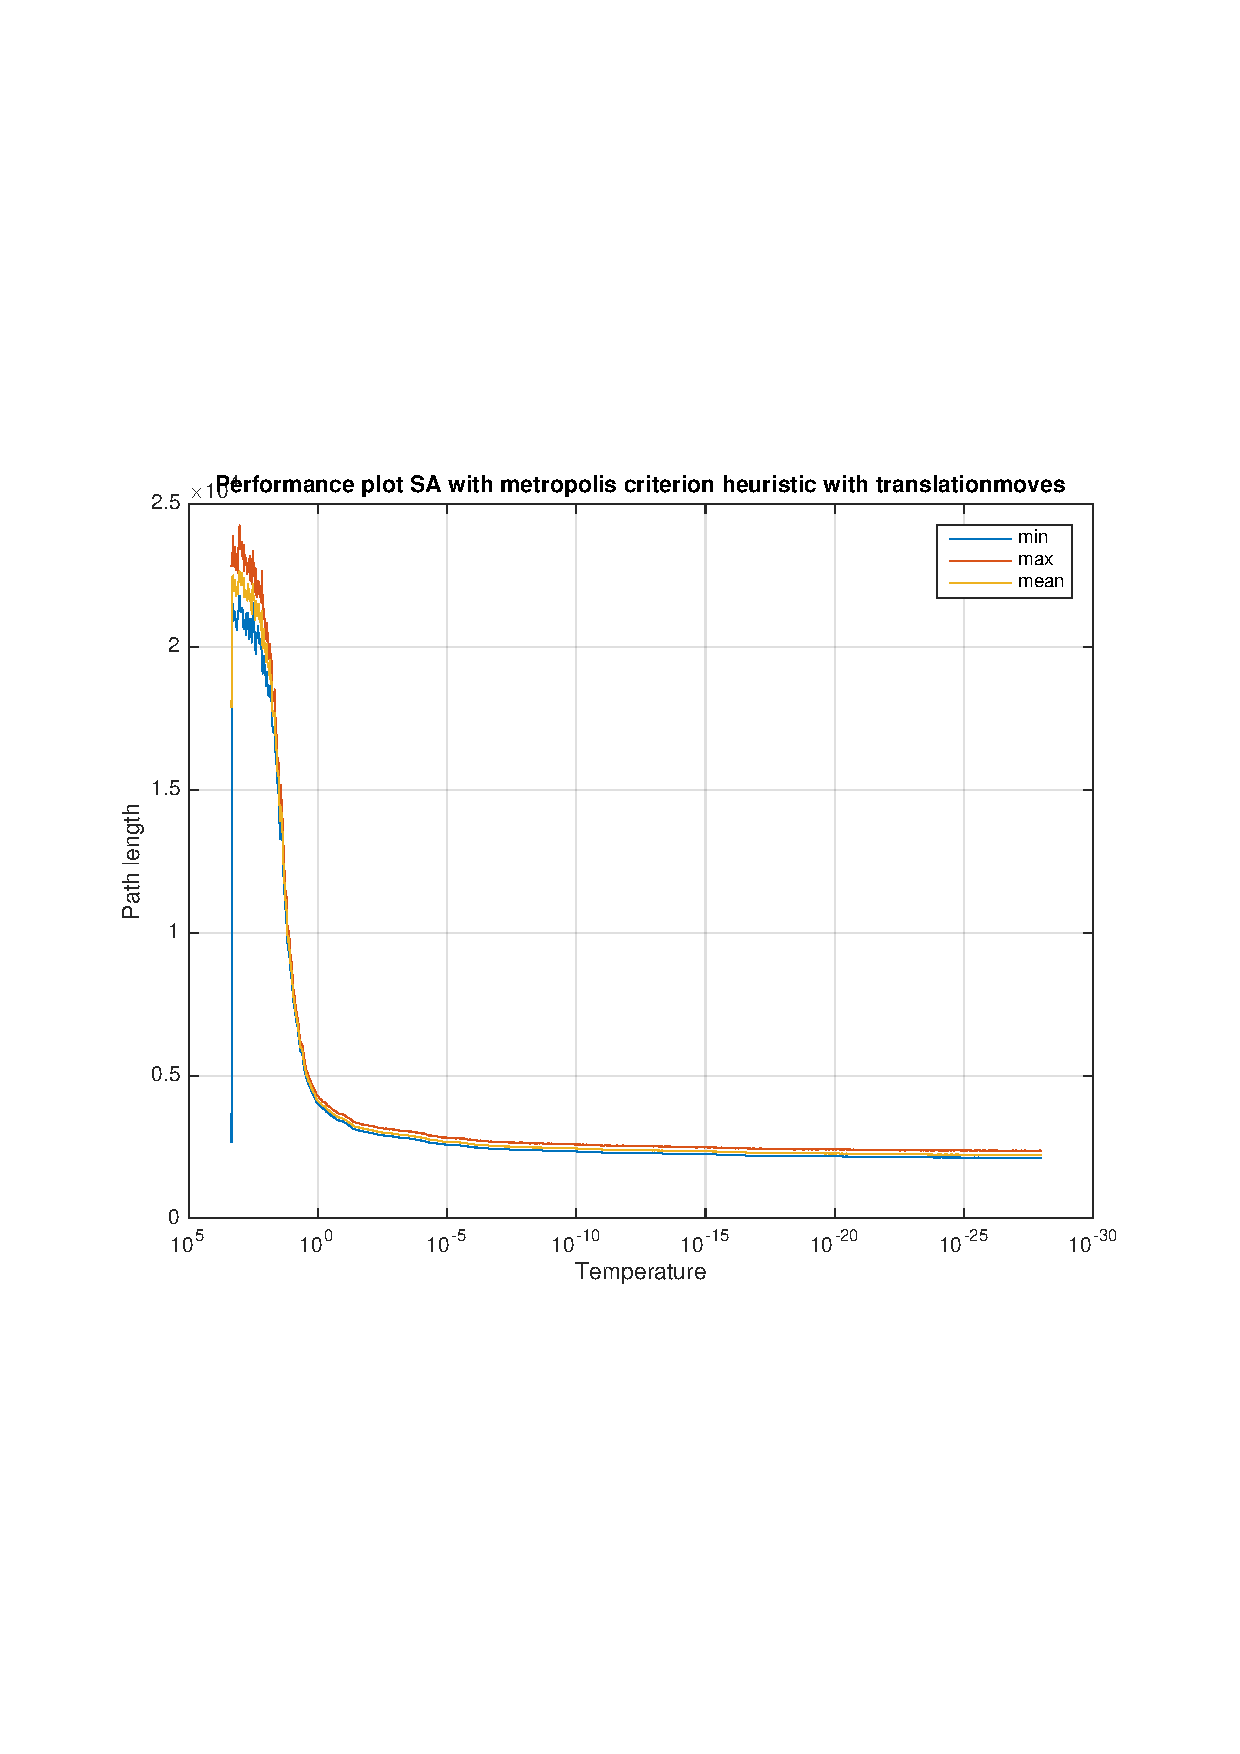
\includegraphics[scale=0.4, trim={3cm 6cm 1cm 6cm}]{../figures/perfPlot_SA_metropolis_translation.pdf} \\ 
    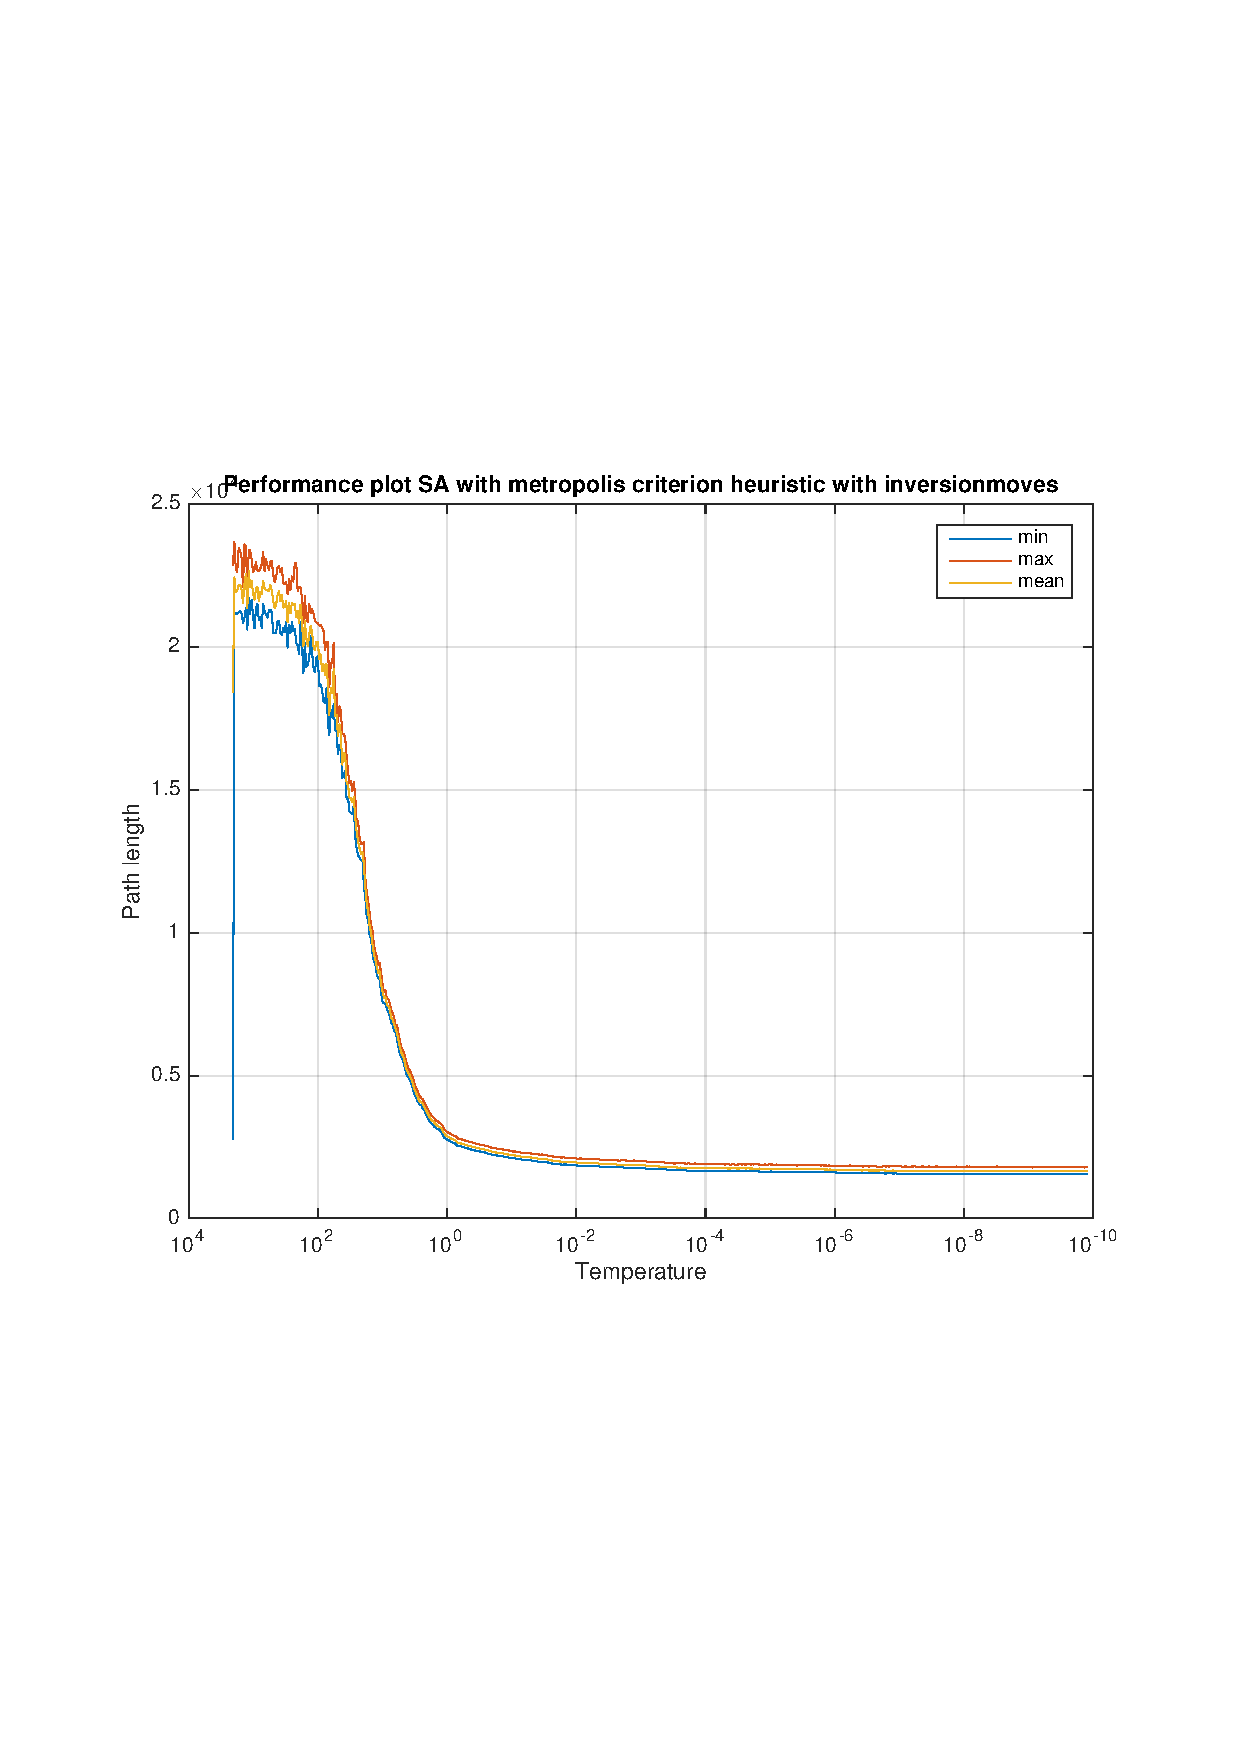
\includegraphics[scale=0.4, trim={3cm 6cm 1cm 6cm}]{../figures/perfPlot_SA_metropolis_inversion.pdf} & 
    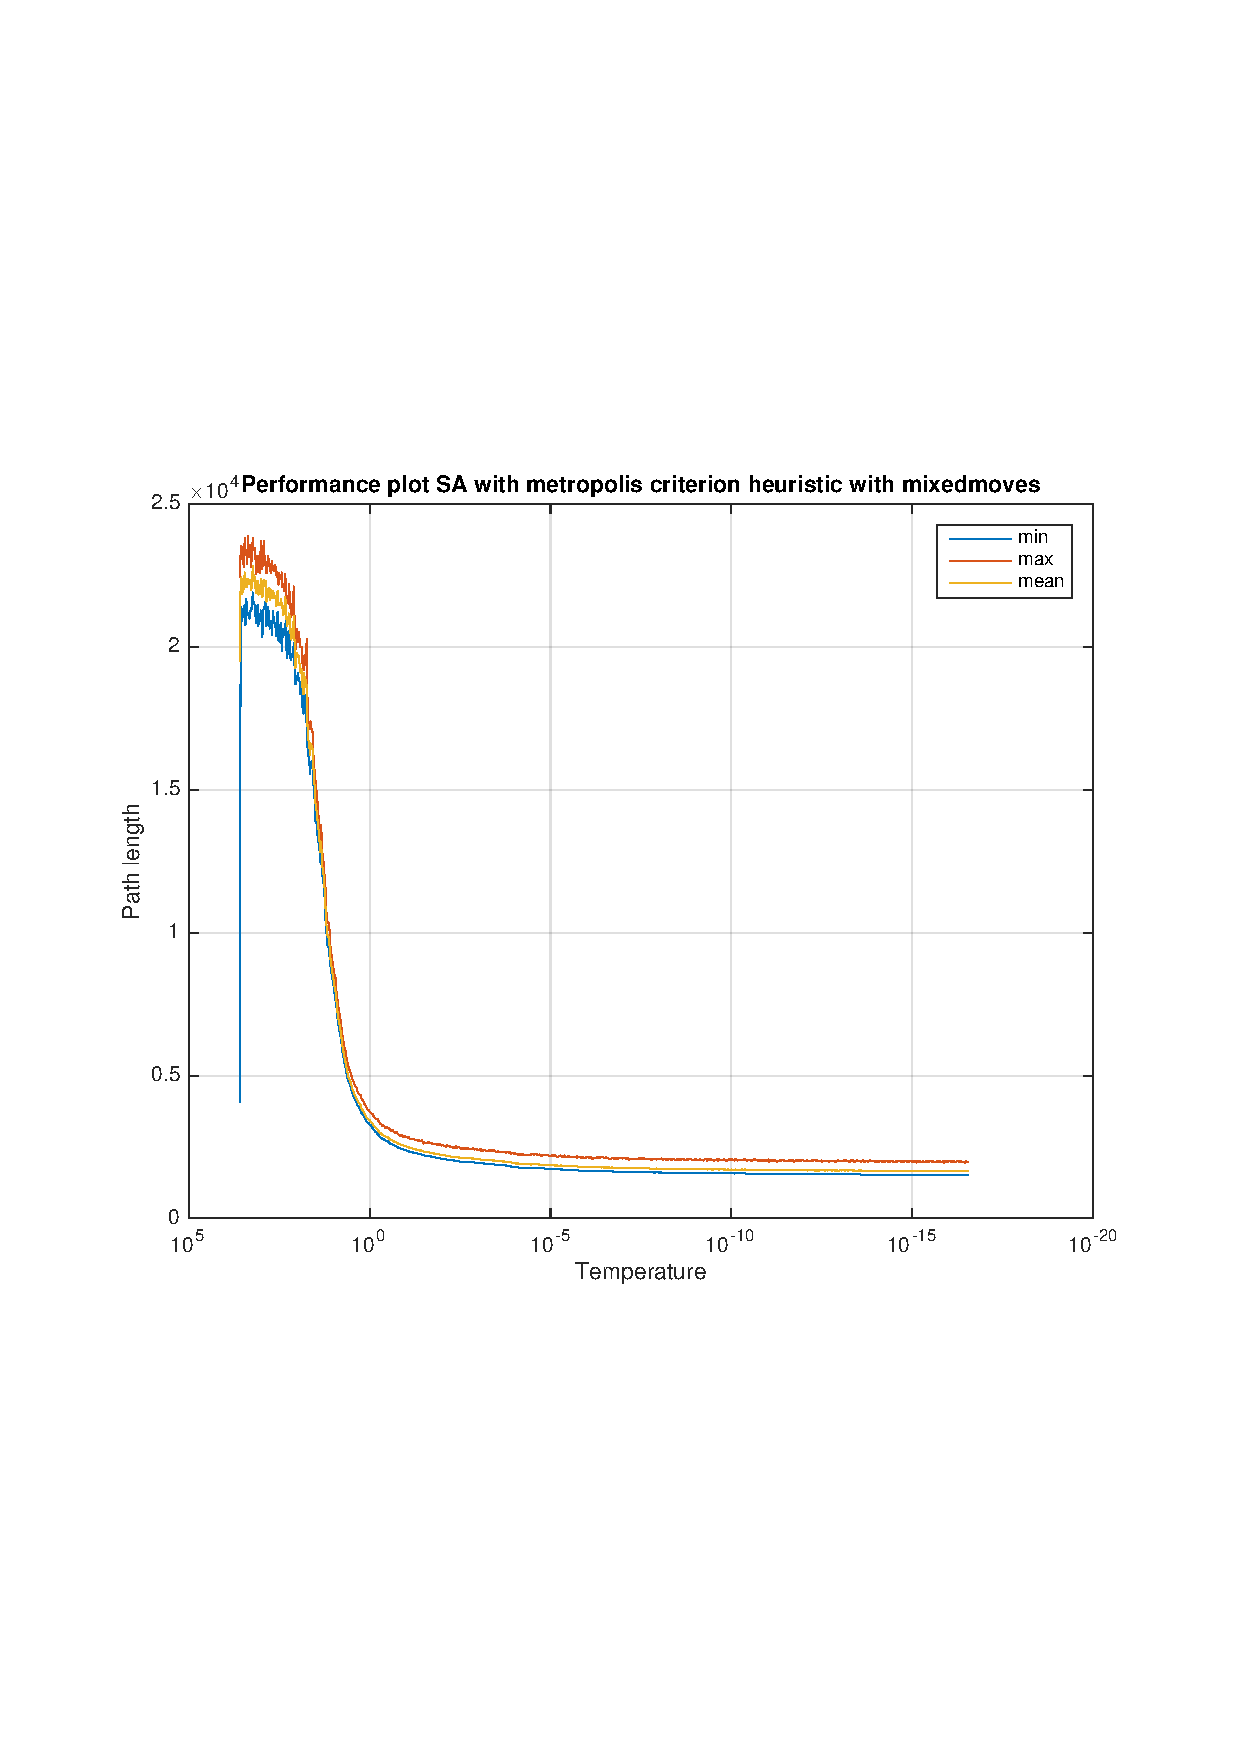
\includegraphics[scale=0.4, trim={3cm 6cm 1cm 6cm}]{../figures/perfPlot_SA_metropolis_mixed.pdf}
  \end{tabular}
  \caption{Performance plots for the SA algorithm with the metropolis criterion}
  \label{fig:perfPlot-SA-metropolis}
\end{figure}

\begin{figure}[!ht]
  \centering
  \begin{tabular}{cc}
    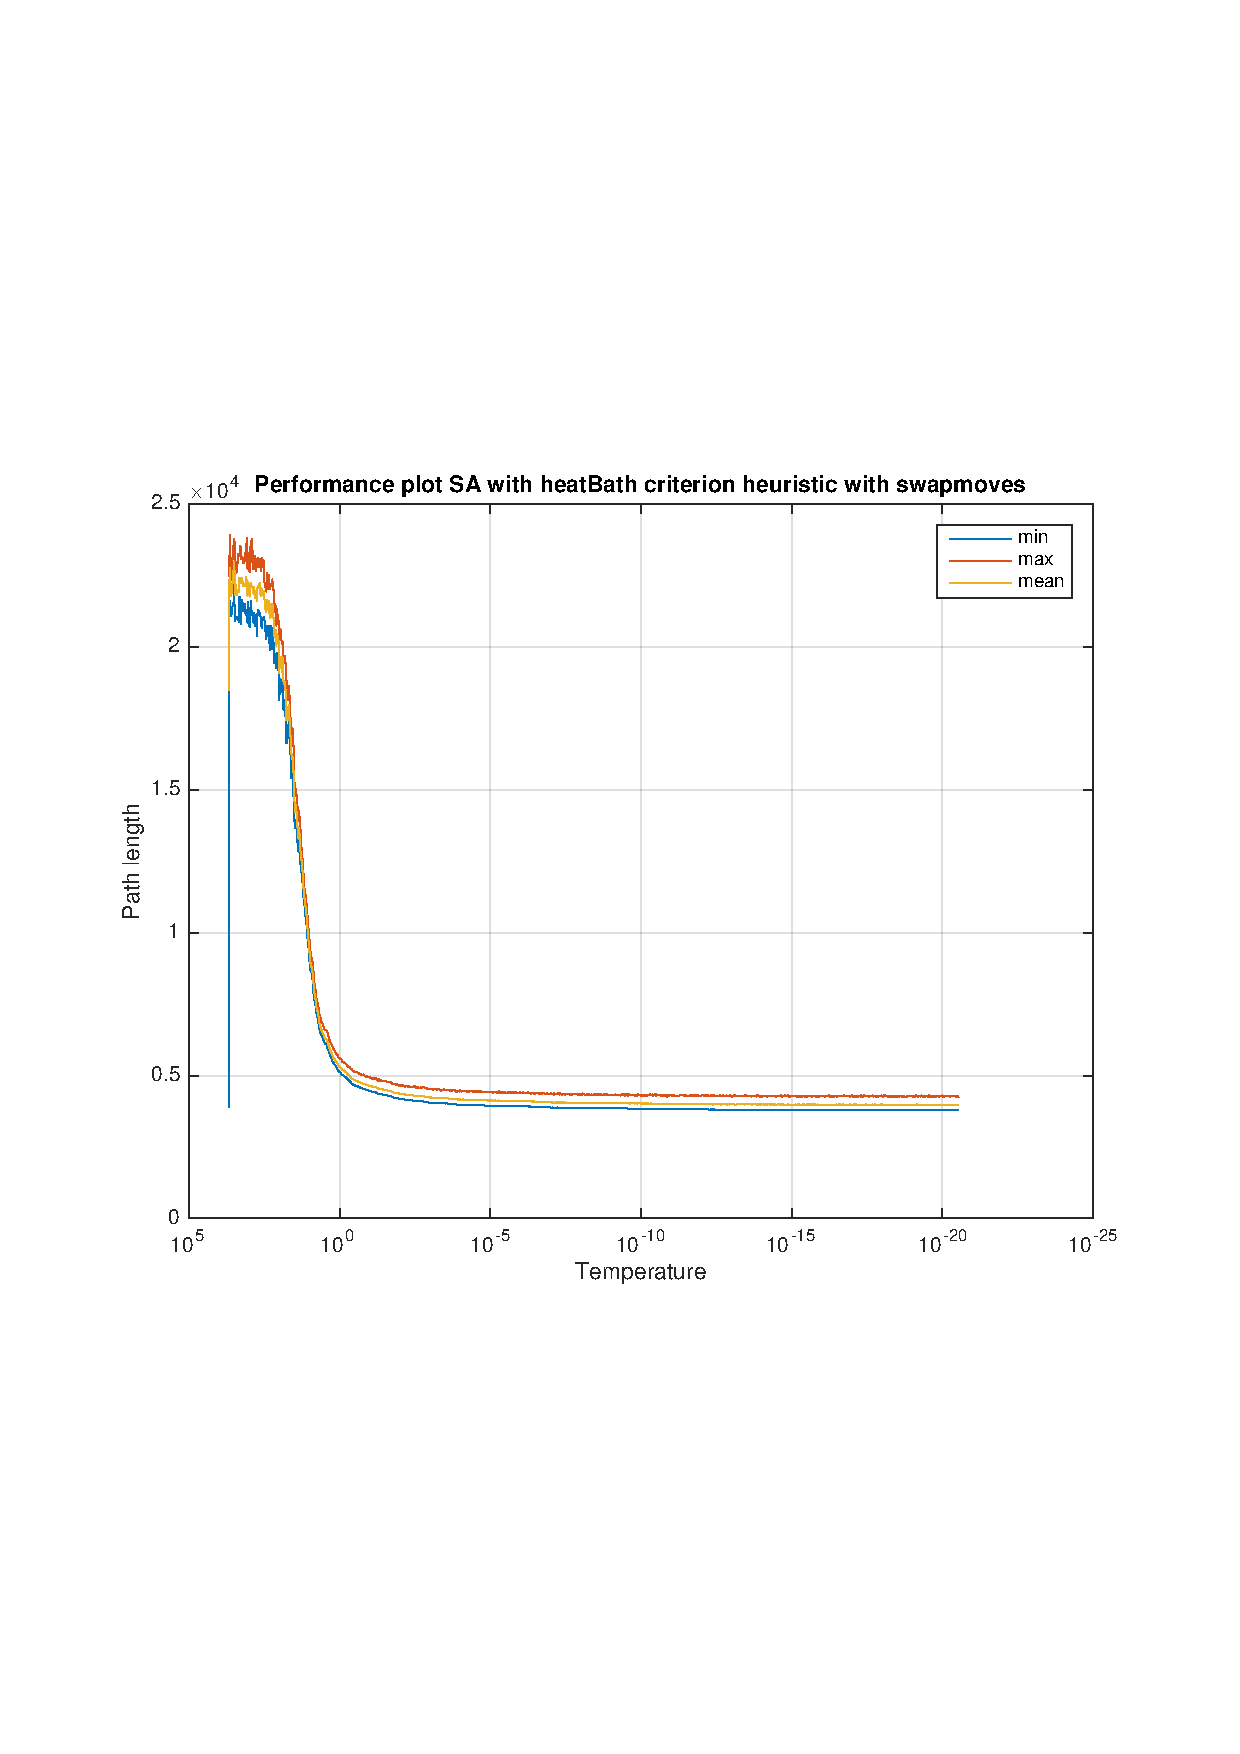
\includegraphics[scale=0.4, trim={3cm 6cm 1cm 6cm}]{../figures/perfPlot_SA_heatBath_swap.pdf} & 
    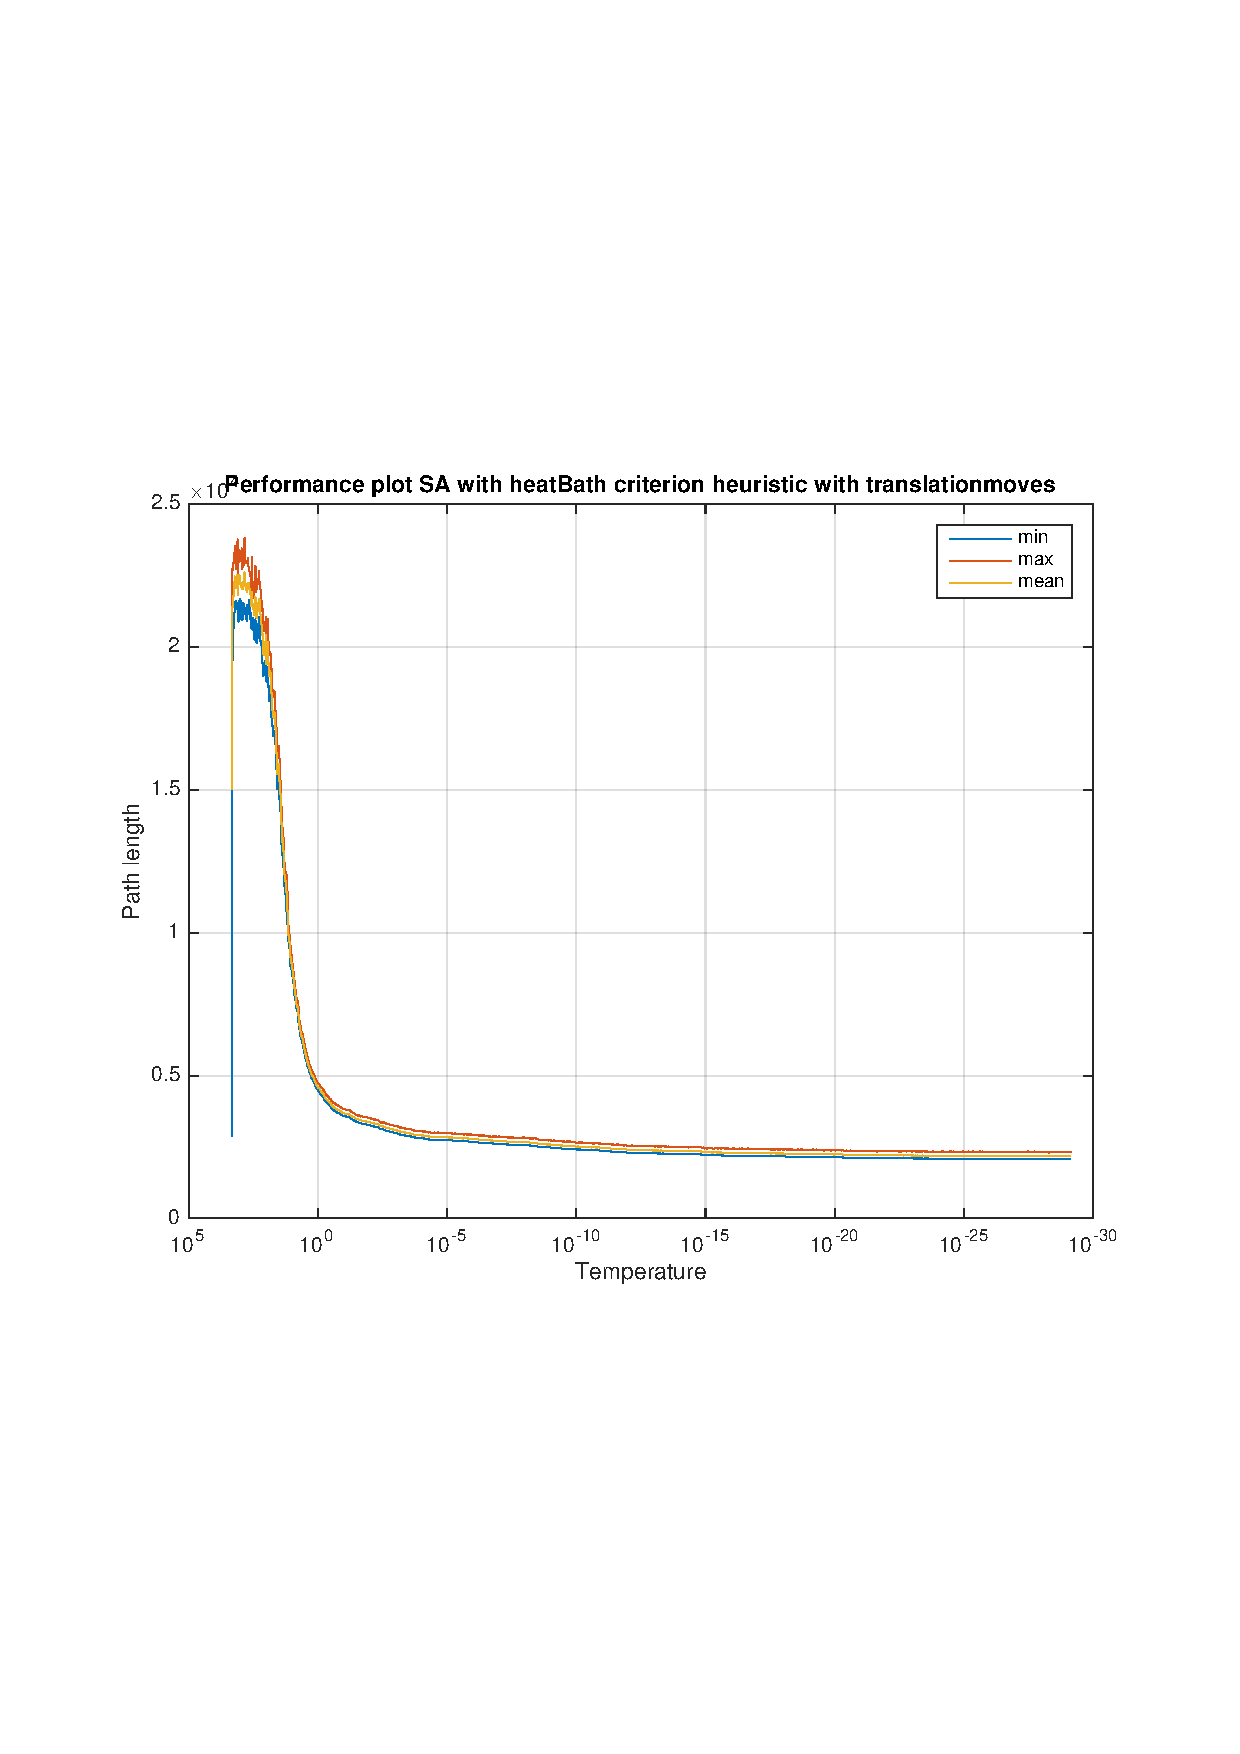
\includegraphics[scale=0.4, trim={3cm 6cm 1cm 6cm}]{../figures/perfPlot_SA_heatBath_translation.pdf} \\ 
    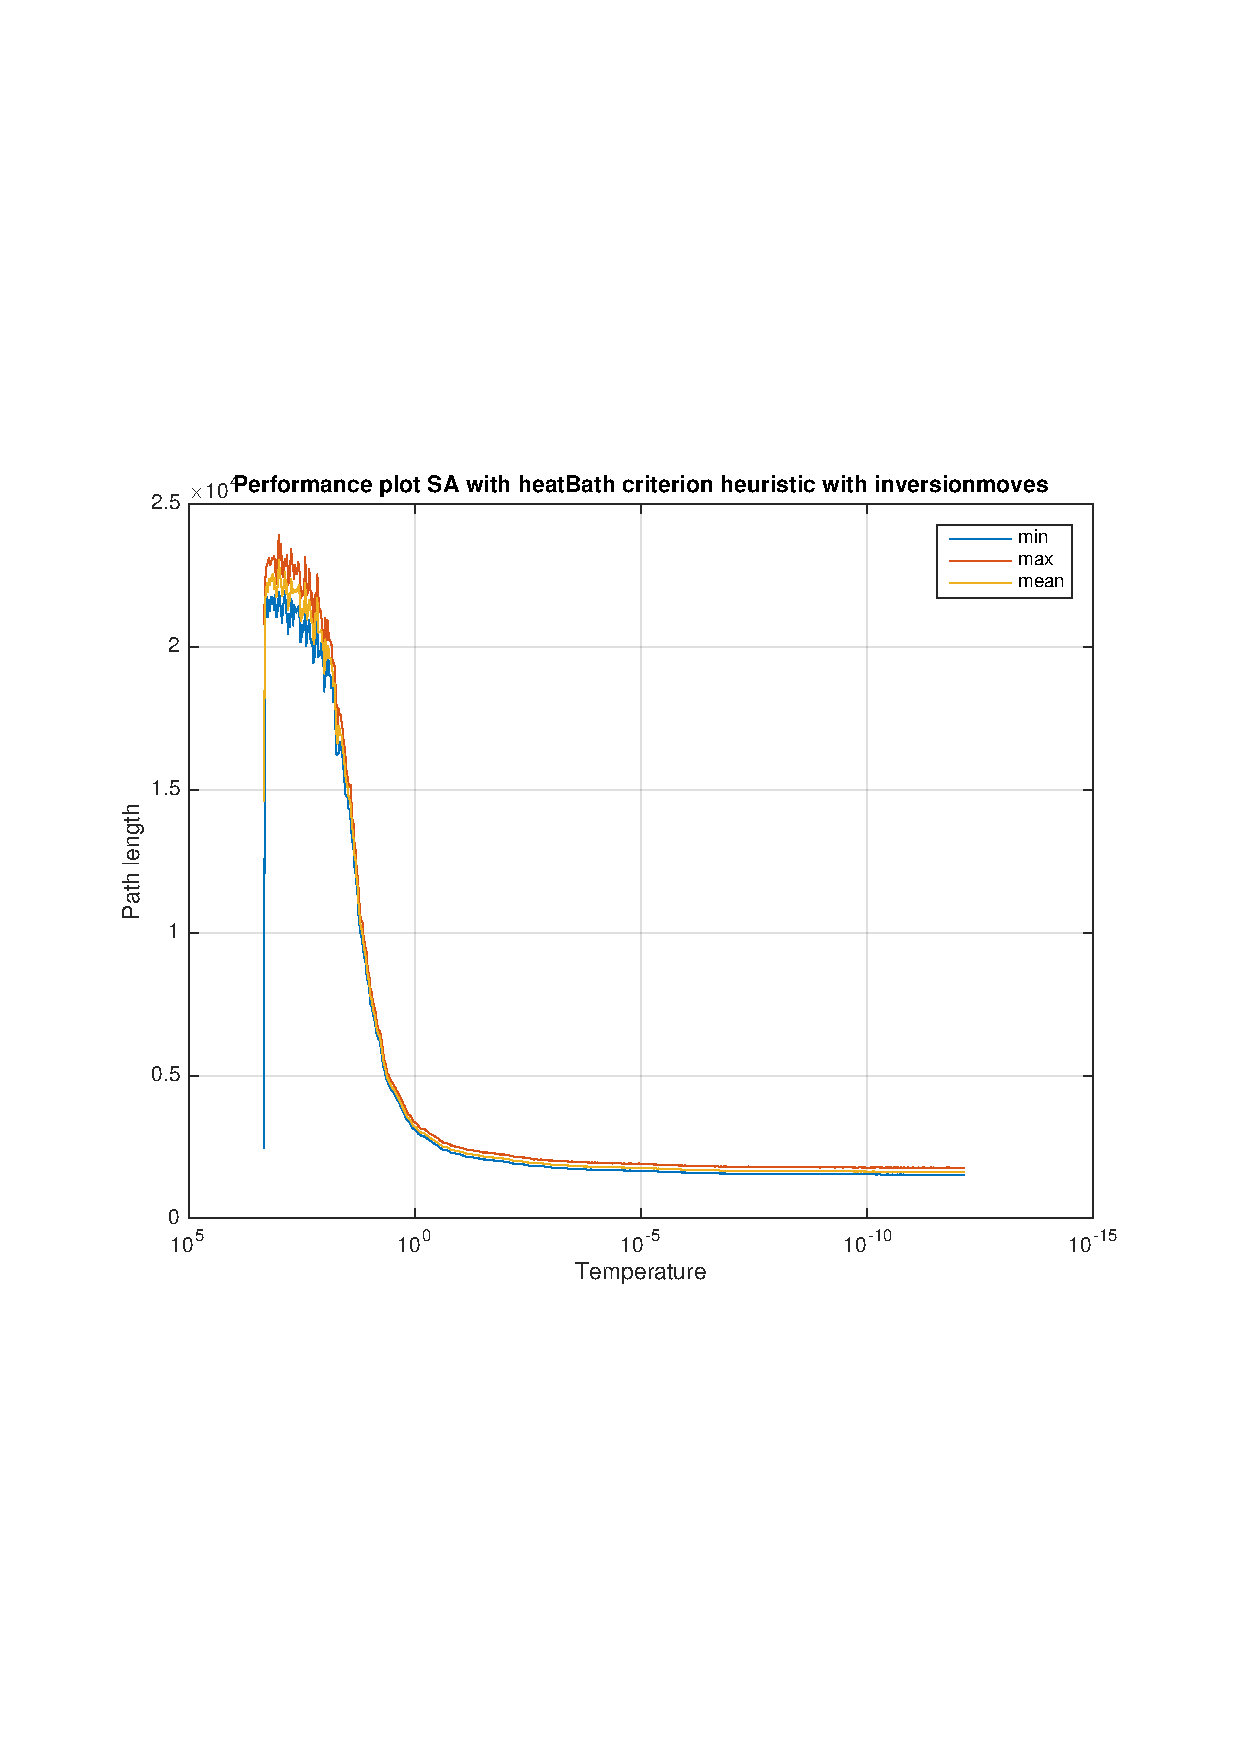
\includegraphics[scale=0.4, trim={3cm 6cm 1cm 6cm}]{../figures/perfPlot_SA_heatBath_inversion.pdf} & 
    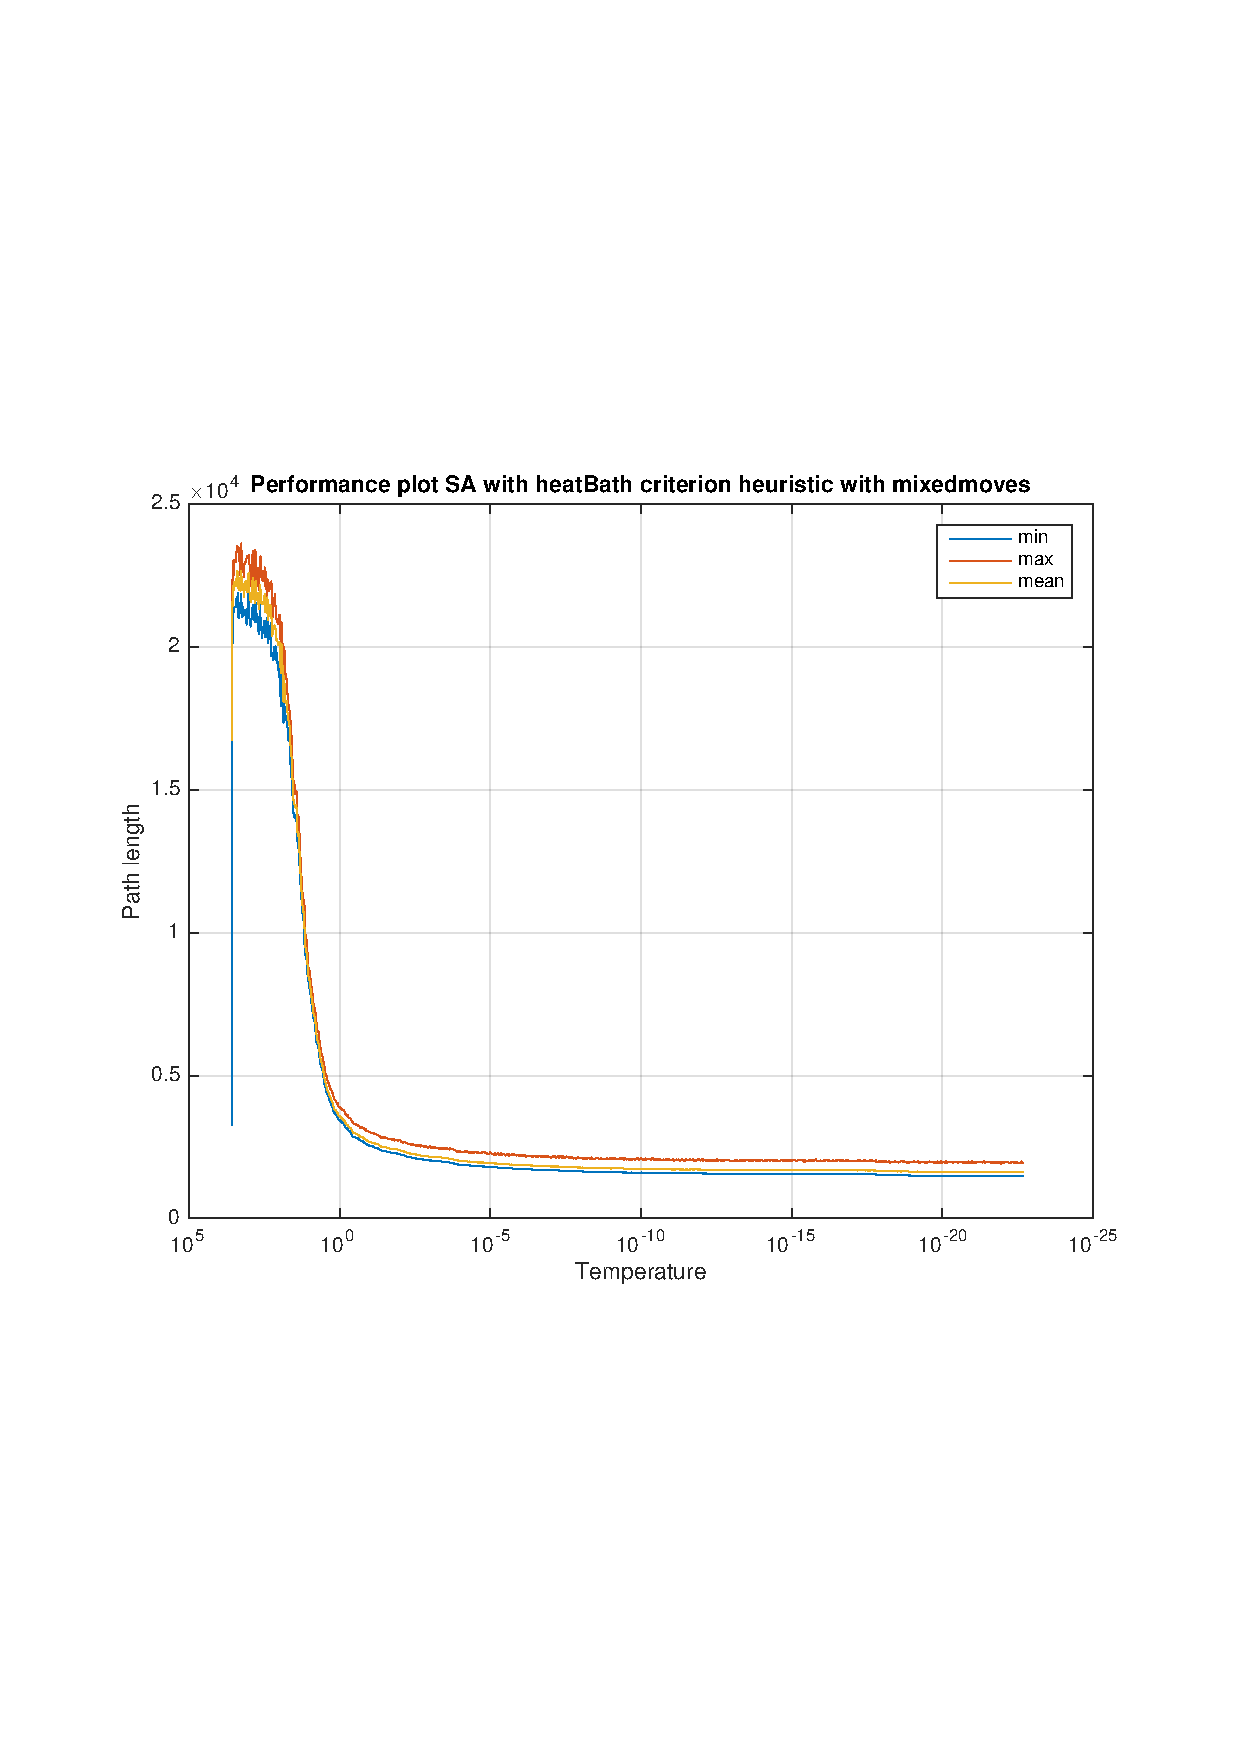
\includegraphics[scale=0.4, trim={3cm 6cm 1cm 6cm}]{../figures/perfPlot_SA_heatBath_mixed.pdf}
  \end{tabular}
  \caption{Performance plots for the SA algorithm with the heat bath condition}
  \label{fig:perfPlot-SA-heatBath}
\end{figure}


\section{Pairwise comparison of algorithms}
\label{sec:pairw-comp-algor}

In this section, we will compare the algorithms we used by making statistical tests. We will use the following
statistical test. We denote by $T$ the statistic 
\[ T = \frac{\overline{x} - \overline{y}}{\sqrt{\frac{\sigma_X^2}{n_X} + \frac{\sigma_Y^2}{n_Y}}}, \]
where $T$ follows a Student distribution $(t_m)$ with $m$ degrees of freedom, where 
\[ m = \frac{\left( \frac{\sigma_X^2}{n_X} + \frac{\sigma_Y^2}{n_Y}
    \right)^2}{\frac{(\sigma_X^2/n_X)^2}{n_X+1} + \frac{(\sigma_Y^2/n_Y)^2}{n_Y+1}} - 2. \]
The acceptance interval is $[-\beta, \beta]$ where 
\[ \beta = t_m^{\alpha / 2} \sqrt{\frac{\sigma_X^2}{n_X} + \frac{\sigma_Y^2}{n_Y}}. \]
In our case we choose $\alpha = 0.5$. 

The results are shown in Table \ref{table:pairwise-comparison}.

\begin{table}[h]
\centering
\caption{Pairwise comparison}
\label{table:pairwise-comparison}
\begin{tabular}{@{}llllll@{}}
\toprule
Algorithms                      & $\mu_X$     & $\mu_Y$    & $T$        & $\beta$ & Best algorithm\\ \midrule
best insertion vs shortest edge & 1521.2787   & 1673.6961  & -19.3326   & 5.3528   & Best insertion\\
metropolis vs heat bath         & 1526.7489   & 1521.7953  & 0.80944  &  4.1537 & Equivalent  \\ \bottomrule
\end{tabular}
\end{table}

We see that the simulated annealing achieves more or less the same performance whether we use the metropolis
condition, or the heat bath criterion. However, the best insertion heuristic is more powerful than the
shortest edge heuristic. 



	
\end{document}



%%% Local Variables:
%%% mode: latex
%%% TeX-master: t 
%%% End: